\documentclass[12pt]{article}\usepackage[]{graphicx}\usepackage[]{color}
%% maxwidth is the original width if it is less than linewidth
%% otherwise use linewidth (to make sure the graphics do not exceed the margin)
\makeatletter
\def\maxwidth{ %
  \ifdim\Gin@nat@width>\linewidth
    \linewidth
  \else
    \Gin@nat@width
  \fi
}
\makeatother

\definecolor{fgcolor}{rgb}{0.345, 0.345, 0.345}
\newcommand{\hlnum}[1]{\textcolor[rgb]{0.686,0.059,0.569}{#1}}%
\newcommand{\hlstr}[1]{\textcolor[rgb]{0.192,0.494,0.8}{#1}}%
\newcommand{\hlcom}[1]{\textcolor[rgb]{0.678,0.584,0.686}{\textit{#1}}}%
\newcommand{\hlopt}[1]{\textcolor[rgb]{0,0,0}{#1}}%
\newcommand{\hlstd}[1]{\textcolor[rgb]{0.345,0.345,0.345}{#1}}%
\newcommand{\hlkwa}[1]{\textcolor[rgb]{0.161,0.373,0.58}{\textbf{#1}}}%
\newcommand{\hlkwb}[1]{\textcolor[rgb]{0.69,0.353,0.396}{#1}}%
\newcommand{\hlkwc}[1]{\textcolor[rgb]{0.333,0.667,0.333}{#1}}%
\newcommand{\hlkwd}[1]{\textcolor[rgb]{0.737,0.353,0.396}{\textbf{#1}}}%

\usepackage{framed}
\makeatletter
\newenvironment{kframe}{%
 \def\at@end@of@kframe{}%
 \ifinner\ifhmode%
  \def\at@end@of@kframe{\end{minipage}}%
  \begin{minipage}{\columnwidth}%
 \fi\fi%
 \def\FrameCommand##1{\hskip\@totalleftmargin \hskip-\fboxsep
 \colorbox{shadecolor}{##1}\hskip-\fboxsep
     % There is no \\@totalrightmargin, so:
     \hskip-\linewidth \hskip-\@totalleftmargin \hskip\columnwidth}%
 \MakeFramed {\advance\hsize-\width
   \@totalleftmargin\z@ \linewidth\hsize
   \@setminipage}}%
 {\par\unskip\endMakeFramed%
 \at@end@of@kframe}
\makeatother

\definecolor{shadecolor}{rgb}{.97, .97, .97}
\definecolor{messagecolor}{rgb}{0, 0, 0}
\definecolor{warningcolor}{rgb}{1, 0, 1}
\definecolor{errorcolor}{rgb}{1, 0, 0}
\newenvironment{knitrout}{}{} % an empty environment to be redefined in TeX

\usepackage{alltt}
% \usepackage{geometry}                % See geometry.pdf to learn the layout options. There are lots.
% \geometry{letterpaper}                   % ... or a4paper or a5paper or ... 
%\usepackage{graphicx}
\usepackage{subcaption}
\usepackage{afterpage}
\usepackage{amssymb}
\usepackage{natbib}
\usepackage{amsmath}
\usepackage{amsfonts}
% \usepackage{color}
\usepackage{multirow}
\usepackage{rotating}
\usepackage[dvipsnames,svgnames,table]{xcolor}
\usepackage{hyperref}
\graphicspath{{figure/}}

\DeclareGraphicsRule{.tif}{png}{.png}{`convert #1 `dirname #1`/`basename #1 .tif`.png}
\usepackage[colorinlistoftodos]{todonotes}
%---------------------------------------------------
%                 Editing Commands
\newcommand{\done}[2][inline]{\todo[color=SpringGreen, #1]{#2}}  % for todos that have been seen and dealt with
\newcommand{\meh}[2][inline]{\todo[color=White, #1]{#2}}   % for todos that may no longer be relevant 
\newcommand{\comment}[2][inline]{\todo[color=SkyBlue, #1]{#2}} % for comments that may not be "to-do"s
%\newcommand{\mcomment}[1]{\todo[color=SkyBlue]{#1}} % for margin comments
\newcommand{\newtext}[1]{\todo[inline, color=White]{ \color{OliveGreen}{#1}}} % new text - not necessarily something to be done
\newcommand{\newdo}[1]{\todo[inline, color=Lime]{#1}} % new to do item
%
%---------------------------------------------------
%                 Placing Figures


%---------------------------------------------------
% Define new environment
\newtheorem{theorem}{Theorem}[section]
\newtheorem{algorithm}[theorem]{Algorithm}
%---------------------------------------------------

%\pdfminorversion=4
% NOTE: To produce blinded version, replace "0" with "1" below.
\newcommand{\blind}{0}

% DON'T change margins - should be 1 inch all around.
\addtolength{\oddsidemargin}{-.5in}%
\addtolength{\evensidemargin}{-.5in}%
\addtolength{\textwidth}{1in}%
\addtolength{\textheight}{1.3in}%
\addtolength{\topmargin}{-.8in}%
\IfFileExists{upquote.sty}{\usepackage{upquote}}{}
\begin{document}

%\bibliographystyle{natbib}

\def\spacingset#1{\renewcommand{\baselinestretch}%
{#1}\small\normalsize} \spacingset{1}


%%%%%%%%%%%%%%%%%%%%%%%%%%%%%%%%%%%%%%%%%%%%%%%%%%%%%%%%%%%%%%%%%%%%%%%%%%%%%%

\if0\blind
{
  \title{\bf Clusters beat Trend!? \\Testing feature hierarchy in statistical graphics}
  \author{Susan VanderPlas\thanks{
    The authors gratefully acknowledge \textit{please remember to list all relevant funding sources in the unblinded version}}\hspace{.2cm}\\
    Department of Statistics and Statistical Laboratory, Iowa State University\\
    and \\
    , Heike Hofmann\\
    Department of Statistics and Statistical Laboratory, Iowa State University}
  \maketitle
} \fi

\if1\blind
{
  \bigskip
  \bigskip
  \bigskip
  \begin{center}
    {\LARGE\bf Clusters beat Trend!? \\Testing feature hierarchy in statistical graphics}
\end{center}
  \medskip
} \fi

\bigskip
\begin{abstract}
Graphics are very effective for communicating numerical information quickly and efficiently, but many of the design choices we make are based on subjective measures, such as personal taste or conventions of the discipline rather than objective criteria. We briefly introduce perceptual principles such as preattentive features and gestalt heuristics, and then discuss the design and results of a factorial experiment designed to examine the effect of plot aesthetics such as color and trend lines on participants' assessment of ambiguous data displays. The quantitative and qualitative experimental results strongly suggest that plot aesthetics have a significant impact on the perception of important features in data displays. 
\end{abstract}

\noindent%
{\it Keywords:}  3 to 6 keywords, that do not appear in the title
\vfill

\newpage
\spacingset{1.45} % DON'T change the spacing!

\tableofcontents
\newpage
\section{Introduction and Background}
Numerical information can be difficult to communicate effectively in raw form, due to limits on attention span, short term memory, and information storage mechanisms within the human brain. 
Graphics are much more effective for communicating numerical information, as (well-designed) graphics order the numerical information spatially and utilize the higher-bandwidth visual system. 
Visual data displays serve as a form of external cognition \citep{zhang1997nature,scaife1996external}, ordering and visually summarizing data which would be hopelessly confusing in tabular format. 
One fantastic example of this phenomenon is the Hertzsprung-Russell (HR) diagram, which was described as ``one of the greatest observational syntheses in astronomy and astrophysics" because it allowed astronomers to clearly relate the absolute magnitude of a star to its' spectral classification; facilitating greater understanding of stellar evolution \citep{spence1993remarkable}. 
The data it displayed was previously available in several different tables; when plotted on the same chart, information that was invisible in a tabular representation became immediately clear \citep{lewandowsky1989perception}. 
Graphical displays more efficiently utilize cognitive resources by reducing the burden of storing, ordering, and summarizing raw data; this frees bandwidth for higher levels of information synthesis, allowing observers to note outliers, understand relationships between variables, and form new hypotheses.

Graphical displays are powerful because they efficiently and effectively convey numerical information, but there exists  relatively sparse empirical information about how the human perceptual system processes these displays. Our understanding of the perception of statistical graphics is informed by general psychological and psychophysics research as well as more specific research into the perception of data displays \citep{cleveland:1984}. 

One relevant focus of psychological research is pre-attentive perception, that is, perception which occurs automatically in the first 200 ms of exposure to a visual stimulus \citep{treisman1985preattentive}. 

Research into {\bf preattentive perception} provides us with some information about the temporal hierarchy of graphical feature processing. Color, line orientation, and shape are processed preattentively; that is, within 200 ms, it is possible to identify a single target in a field of distractors, if the target differs with respect to color or shape \citep{goldstein2009encyclopedia}. 
Research by \citet{healey1999large} extends this work, demonstrating that certain features of three-dimensional data displays are also processed preattentively. However, neither target identification nor three-dimensional data processing always translate into faster or more accurate inference about the data displayed, particularly when participants have to integrate several preattentive features to understand the data. 

{\bf Feature detection} at the attentive stage of perception has also been examined in the context of statistical graphics; researchers have evaluated the perceptual implications of utilizing color, fill, shapes, and letters to denote categorical or stratified data in scatterplots. \citet{cleveland:1984} ranked the optimality of these plot aesthetics based on response accuracy, preferring colors, amount of fill, shapes, and finally letters to indicate category membership. \citet{lewandowsky1989discriminating} examined both accuracy and response time, finding that color is faster and more accurately perceived (except by individuals with color deficiency). Shape, fill, and discriminable letters (letters which do not share visual features, such as HQX) were identified as less accurate than color, while confusable letters (such as HEF) result in significantly decreased accuracy. 

{\bf Gestalt psychology} is another area of psychological research, that examines perception as a holistic experience, establishing and evaluating mental heuristics used to transform visual stimuli into useful, coherent information. 
Gestalt rules of perception can be easily applied to statistical graphics, as they describe the way we organize visual input, focusing on the holistic experience rather than the individual perceptual features. 

For example, rather than perceiving four legs, a tail, two eyes, two ears, and a nose, we perceive a dog. This is due to certain perceptual heuristics, which provide a ``top-down" method of understanding visual stimuli by taking into account past experience. 

The rules of perceptual organization relevant to graphical perception in this experiment are:
\begin{itemize}
\item \textbf{Proximity}: two elements which are close together are more likely to belong to a single unit.
\item \textbf{Similarity}: the more similar two elements are, the more likely they belong to a single unit.
\item \textbf{Good continuation}: two elements which blend together smoothly likely belong to one unit.
\item \textbf{Common region}: elements contained within a common region likely belong together. 
\end{itemize}
A complete list of the rules of perceptual grouping can be found in \citet{goldstein2009encyclopedia}.


\begin{figure}\centering
\begin{knitrout}
\definecolor{shadecolor}{rgb}{0.969, 0.969, 0.969}\color{fgcolor}

{\centering \includegraphics[width=0.32\linewidth]{figure/gestalt1-1} 
\includegraphics[width=0.32\linewidth]{figure/gestalt1-2} 
\includegraphics[width=0.32\linewidth]{figure/gestalt1-3} 

}



\end{knitrout}
\caption[Gestalt principles applied to statistical plots]{\label{fig:gestalt} \emph{Proximity} renders the fifty points of the first scatterplot as two distinct (and equal-sized) groups. Shapes and colors create different groups of points in the middle scatterplot, invoking the Gestalt principle of \emph{Similarity}. \emph{Good Continuation} renders the points in the scatterplot on the right hand side into two groups of points on curves: one a straight line with an upward slope, the other a curve that initially decreases and at the end of the range shows an uptick.} 
\end{figure}
% \afterpage{\clearpage}

The plots in Figure~\ref{fig:gestalt} demonstrate several of the gestalt principles which combine to order our perceptual experience from the top down. These laws help to order our perception of charts as well: points which are colored or shaped the same are perceived as belonging to a group (similarity), points within a bounding interval or ellipse are perceived as belonging to the same group (common region), and regression lines with confidence intervals are perceived as single units (continuity and common region). 

The processing of visual stimuli utilizes low-level feature detection, which occurs automatically in the preattentive perceptual phase, and higher-level mental heuristics which are informed by experience. Both types of mental processes utilize physical location, color, and shape  to organize perceptual stimuli and direct attention to graphical features which stand out. 

Research on preattentive perception is important because features that are perceived preattentively do not require as much mental effort to process from raw visual stimuli; subsequent top-down gestalt heuristics can be applied to the categorized features in order to make sense of the visual scene once the attentive stage of perception is reached. 


This paper describes the results of a user study designed to explore the hierarchy of gestalt principles in perception of statistical graphics. We utilize information from previous studies \citep{heer:2014, robinson:03, healey1996high} concerning the hierarchy of preattentive feature perception in order to maximize the effect of preattentive feature differences. 


Statistical graphics can be difficult to examine experimentally; qualitative studies rely on descriptions of the plot by participants who may not be able to articulate their observations precisely, while quantitative studies may only be able to examine whether the viewer can accurately read numerical information from the chart, instead of exploring the overall utility of the data display holistically. Here, we are describing the setup and results of a study using statistical lineup methodology to provide quantitative and qualitative information.

\paragraph{Statistical lineups} 
are an important experimental tool for evaluating the perceptual utility of graphical displays. Lineups fuse commonly used psychological tests (target identification, visual search) \citep{visualreasoning} with statistical hypothesis tests to facilitate formal experimental evaluation of statistical graphics. 

Lineups are an experimental tool designed to serve as a visual hypothesis test, separating ``significant" visual effects from those that would be expected under a null hypothesis \citep{buja2009statistical, majumder2013validation,hofmann2012graphical, wickham2010graphical}. 
A statistical lineup consists of (usually) 20 sub-plots, arranged in a grid (examples are shown in Figure~\ref{fig:plotExamples}). 
Of these plots, one plot is the ``target plot'', generated from either real data or an alternate model (equivalent to $H_A$ in hypothesis testing); the other 19 plots are generated either using bootstrap samples of the real data or by generating ``true null" plots from the null distribution $H_0$. 
If participants can identify the target plot from the field of distractors, then the visual display is deemed significant in the same sense that a numerical test with $p<0.05$ is significant. 

Apart from the hypothesis testing construct, the use of statistical lineups to test statistical graphics conforms nicely to psychological testing constructs such as visual search \citep{demita1981validity,treisman1980feature}, where a single target is embedded in a field of distractors and response time, accuracy, or both are used to measure the complexity of the underlying psychological processes leading to identification. 

% \comment{Should the next 3 paragraphs go into a different section? Otherwise, the "Intro" part in the last paragraph gets hidden under the "Statistical Lineups" heading...}

In this paper we {\bf modify the lineup protocol} by introducing a second target to each lineup. The two targets represent two different, competing signals; an observer's choice then demonstrates empirically which signal is more salient. 
If both targets exhibit similar signal, observers may identify both targets, removing any forced-choice scenario which might skew results in a study. % (few participants exercised this option). 

By tracking the proportion of observers choosing either target plot (a measure of overall lineup difficulty) as well as which proportion of observers choose one target over the other target, we can determine the relative strength of the two competing signals amid a field of distractors. At this level, signal strength is determined by the experimental data and the generating model; we are measuring the ``power" (in a statistical sense) of the human perceptual system, rather than raw numerical signal. 

Using this testing framework, we  apply different aesthetics, such as color and shape, as well as plot objects which display statistical calculations, such as trend lines and bounding ellipses. These additional plot layers, discussed in more detail in the next section, are designed to emphasize one of the two competing targets and affect the overall visual signal of the target plot relative to the null plots. We expect that in a situation similar to the third plot of Figure~\ref{fig:gestalt}, the addition of two trend lines would emphasize the ``good continuation" of points in the plot, producing a stronger visual signal, even though the underlying data has not changed. Similarly, the grouping effect in the first plot in the Figure~should be enhanced if the points in each group were colored differently, as the proximity heuristic is supplemented by similarity. In plots that are ambiguous, containing some clustering of points as well as a linear relationship between $x$ and $y$, additional aesthetic cues may ``tip the balance" in favor of recognizing one type of signal.

The study in this paper is designed to inform our understanding of the perceptual implications of these additional aesthetics, in order to provide guidelines for the creation of data displays which provide visual cues consistent with gestalt heuristics and preattentive perceptual preferences. 

The next section discusses the particulars of the experimental design, including the data generation model, plot aesthetics, selection of color and shape palettes, and other important considerations. Experimental results are presented in section \ref{sec:Results}, and implications and conclusions are discussed in section \ref{sec:Conclusion}. 

\section{Experimental Setup and Design} \label{sec:ExperimentalDesign}
In this section, we discuss the generating data models for the two types of signal plots and the null plots, the selection of plot aesthetic combinations and aesthetic values, and the design and execution of the experiment.

\subsection{Data Generation}
Lineups require a single ``target" data set (which we are expanding to two competing ``target" data sets), and a method for generating null plots. When utilizing real data for target plots, null plots are often generated through permutations.

Here, it is possible to generate true null plots, which are generated from the null model and do not depend on the data used in the target plot. 
This experiment will measure two competing gestalt heuristics, proximity and good continuation, using two data-generating models: $M_C$, which generates data with $K$ clusters, and $M_T$, which generates data with a positive correlation between $x$ and $y$. 
True null datasets are created using a mixture model $M_0$ which combines $M_C$ and $M_T$. Both $M_C$ and $M_T$ generate data in the same range of values. 
Additionally, $M_C$ generates clustered data with linear correlations that are within $\rho = (0.25, 0.75)$, similar to the linear relationship between datasets generated by $M_0$, and $M_T$ generates data with clustering similar to $M_0$. These constraints provide some assurance that participants who select a plot with data generated from $M_T$ are doing so because of visual cues indicating a linear trend (rather than a lack of clustering compared to plots with data generated from $M_0$), and participants who select a plot with data generated from $M_C$ are doing so because of visual cues indicating clustering, rather than a lack of a linear relationship relative to plots with data generated from $M_0$. 


\subsubsection{Regression Model \texorpdfstring{$M_T$}{Mt}}
This model has the parameter $\sigma_T$ to reflect the amount of scatter around the trend line. It generates $N$ points $(x_i, y_i), i=1, ..., N$ where $x$ and $y$ have a positive linear relationship. The data generation mechanism is as follows: 

\begin{algorithm}\hfill\newline
  Input Parameters: sample size $N$, $\sigma_T$ standard deviation around the line \\
  Output: $N$ points, in form of vectors $x$ and $y$.
  \begin{enumerate}
    \item Generate $\tilde{x}_i$, $i=1, ..., N$, as a sequence of evenly spaced points from $[-1, 1]$. 
    \item Jitter $\tilde{x}_i$ by adding small uniformly distributed perturbations to each of the values: $x_i = \tilde{x}_i + \eta_i$, where $\eta_i \sim \text{Unif}(-z, z)$, $z = \frac{2}{5(N-1)}$.
    \item Generate $y_i$ as a linear regressand of $x_i$: $y_i = x_i + e_i$, $e_i \sim N(0, \sigma^2_T)$.
    \item Center and scale $x_i$, $y_i$.
  \end{enumerate}
\end{algorithm}

We compute the coefficient of determination for all of the plots to assess the amount of linearity in each panel, computed as 
\begin{equation}\label{eq:linearMeasure}
R^2 = 1 - \frac{RSS}{TSS},
\end{equation}
where TSS is the total sum of squares, $TSS = \sum_{i=1}^N \left(y_i - \bar{y}\right)^2$ and $RSS = \sum_{i=1}^N e_i^2$, the residual sum of squares.
The expected value of the coefficient of determination $E\left[R^2\right]$ in this scenario is 
\[
E\left[R^2\right] =  \frac{1}{1 + 3\sigma^2_T},
\]
because
$E[RSS] = N\sigma^2_T$ and $E[TSS] = \sum_{i=1}^N E\left[y_i^2\right]$  (as $E[Y] = 0$), where 
$$
E\left[y_i^2\right] = E\left[x_i^2 + e_i^2 + 2 x_ie_i\right] = \frac{1}{3} + \sigma^2_T. 
$$
The use of $R^2$ to assess the strength of the linear relationship (rather than the correlation) is indicated because human perception of correlation strength more closely aligns with $R^2$ \citep{bobko1979perception,lewandowsky1989perception}. 

\begin{figure}[ht]
\begin{knitrout}
\definecolor{shadecolor}{rgb}{0.969, 0.969, 0.969}\color{fgcolor}

{\centering \includegraphics[width=\linewidth]{figure/trends-1} 

}



\end{knitrout}
\caption[Parameters affecting $M_T$]{\label{fig:trends} Set of scatterplots showing one draw each from the trend model $M_T$ for parameter values of  $\sigma_T \in \{0.1, 0.2, 0.3, 0.4\}$.}
\end{figure}

\subsubsection{Cluster Model \texorpdfstring{$M_C$}{Mc}} 
We begin by generating $K$ cluster centers on a $K \times K$ grid, then we generate points around selected cluster centers. 
\begin{algorithm}\hfill\newline
  Input Parameters:  $N$ points, $K$ clusters, $\sigma_C$ cluster standard deviation \\
  Output: $N$ points, in form of vectors $x$ and $y$. 
  \begin{enumerate}
    \item Generate cluster centers $(c^x_{i}, c^y_{i})$ for each of the $K$ clusters, $i=1, ..., K$:
      \begin{enumerate}
        \item in form of two vectors $c^{x}$ and $c^y$ of permutations of $\{1, ..., K\}$, such that
        \item the correlation between cluster centers \text{cor}$(c^{x}, c^{y})$ falls into a range of $[.25, .75]$.
      \end{enumerate}
      \item Center and standardize cluster centers $(c^x, c^y)$:  
      \[
        \tilde{c}^x_{i} = \frac{c^x_{i} - \bar{c}}{s_c} \ \ \text{ and } \ \ \tilde{c}^y_{i} = \frac{c^y_{i} - \bar{c}}{s_c},
      \]
      where $\overline{c} = (K+1)/2$ and $s_c^2 = \frac{K(K+1)}{12}$ for all $i = 1, ..., K$.
    \item For the $K$ clusters, we want to have nearly equal sized groups, but allow some variability. Cluster sizes  $g = (g_1, ..., g_K)$ with $N = \sum_{i=1}^K g_i$, for clusters $1, ..., K$ are therefore determined as a draw from a multinomial distribution: 
    \[
    g \sim \text{Multinomial }(K, p) \text{ where } p = \tilde{p}/\sum_{i=1}^K \tilde{p}_i, \text{ for } \tilde{p} \sim N \left(\frac{1}{K}, \frac{1}{2 K^2} \right).
    \]
     
    \item Generate points around cluster centers by adding small normal perturbations: 
      \begin{eqnarray*}
        x_i &=& \tilde{c}^x_{g_i} + e^x_i, \text{ where } e^x_i \sim N(0, \sigma^2_C),\\
        y_i &=& \tilde{c}^y_{g_i} + e^y_i, \text{ where } e^y_i \sim N(0, \sigma^2_C).
      \end{eqnarray*}
    \item Center and scale $x_i$, $y_i$.
  \end{enumerate}
\end{algorithm} 

\begin{figure}[bht]
\begin{knitrout}
\definecolor{shadecolor}{rgb}{0.969, 0.969, 0.969}\color{fgcolor}

{\centering \includegraphics[width=\linewidth]{figure/cluster-1} 

}



\end{knitrout}
\caption[Parameters affecting $M_C$]{\label{fig:clusters} Scatterplots of clustering output for different inner cluster spread $\sigma_C$  (left to right) and different number of clusters $K$ (top and bottom), generated using the same random seed at each parameter setting. The colors and shapes shown are those used in the lineups for $K=3$ and $K=5$.}
\end{figure}
As a measure of cluster cohesion we use a coefficient to assess the amount of variability within each cluster, compared to total variability. Note that for the purpose of clustering, variability is measured as the variability in both $x$ and $y$ from a common mean, i.e.\ we implicitly assume that the values in $x$ and $y$ are on the same scale. This ensures that $\sigma_C$is a scaling parameter that regulates the amount of cluster cohesion (see Figure~\ref{fig:clusters}).  % (which we achieve by scaling in the final step of the generation algorithm).


%\afterpage{\clearpage}

\newcomment{$\sigma_C$ is the theoretical regulator of variability, while $C^2$ is the after-the-fact measure of the amount of spread. XXX Do we know the relationship between those two measurements? -- it should be similar to $R^2$ versus $\sigma$.}
For two numeric variables $x$ and $y$ and grouping variable $g$ with $g_i \in \{1, ..., K\}, i = 1, ..., n$, we compute the  {\it cluster index} $C^2$ as follows: let $j(i)$ be the function that maps index $i = 1, ..., n$ to one of the clusters $1, ..., K$ given by the grouping variable $g$. Then for each  level of $g$, we find  a cluster center as $\bar{x}_{j(i)}$ and  $\bar{y}_{j(i)}$, and we determine the strength of the clustering by comparing the within cluster variability with the overall variability: 

\begin{eqnarray}\label{eq:clusterMeasure}
C^2 &=& \frac{CSS}{TSS},\\
\nonumber CSS &=& \sum_{i=1}^n \left(x_{j(i)} - \overline{x}_{j(i)}\right)^2 + \left(y_{j(i)} - \overline{y}_{j(i)} \right)^2, \\
\nonumber TSS &=& \sum_{i=1}^n \left(x_i - \bar{x}\right)^2 + \left(y_i - \bar{y}\right)^2.
\end{eqnarray}


\subsubsection{Null Model \texorpdfstring{$M_0$}{M0}}
The generative model for null data is a mixture model $M_0$ that draws $n_c \sim \text{Binomial}(N, \lambda)$ observations from the cluster model, and $n_T = N - n_c$ from the regression model $M_T$. Observations are assigned to specific clusters using hierarchical clustering, which creates groups consistent with any structure present in the generated data. This provides a plausible grouping for use in aesthetic and statistics requiring categorical data (color, shape, bounding ellipses). 

\begin{figure}[hbt]
\begin{knitrout}
\definecolor{shadecolor}{rgb}{0.969, 0.969, 0.969}\color{fgcolor}

{\centering \includegraphics[width=.9\linewidth]{figure/lambda-1} 

}



\end{knitrout}
\caption[Mixing parameter for null model $M_0$]{\label{fig:lambda} Scatterplots of data generated from $M_0$ using different values of $\lambda$, generated using the same random seed at each $\lambda$ value.}
\end{figure}
%\afterpage{\clearpage}

Null data in this experiment is generated using $\lambda = 0.5$, that is, each point in a null data set is equally likely to have been generated from $M_C$ and $M_T$. 

\subsubsection{Parameters used in Data Generation}
Models $M_C$, $M_T$, and $M_0$ provide the foundation for this experiment; by manipulating cluster standard deviation $\sigma_C$ and regression standard deviation $\sigma_T$ (directly related to correlation strength) for varying numbers of clusters $K=3, 5$, we can systematically control the statistical signal present in the target plots and generate corresponding null plots that are mixtures of the two distributions. For each parameter set $\{K, N, \sigma_C, \sigma_T\}$, as described in table \ref{tab:parameters}, we  generate a lineup dataset consisting of one set drawn from $M_C$, one set drawn from $M_T$, and 18 sets drawn from $M_0$. 

\begin{table}[hbtp]
  \rowcolors{2}{gray!25}{white}
\begin{center}
\begin{tabular}{lll}
\bf Parameter & \bf Description & \bf Choices\\\hline
$K$ & \# Clusters &  \begin{tabular}{l}3, 5 \end{tabular} \\
$N$ & \# Points &  \begin{tabular}{l}$15\cdot K$\end{tabular} \\
$\sigma_T$ & Scatter around trend line &   \begin{tabular}{l}.15, .25, .35  \end{tabular}\\
$\sigma_C$ & Scatter around cluster centers & \begin{tabular}{ll} .25, .30, .35 ($K=3$)\\ .20, .25, .30 ($K=5$) \end{tabular}
\\\hline
\end{tabular}
\end{center}
\caption{Parameter settings for generation of lineup datasets. \label{tab:parameters}}
\end{table}

The parameter values were chosen after examining the full parameter space through simulation of 1000 lineup datasets for each combination of $\sigma_T\in\{0.2, 0.25, ..., 0.5\}$, $\sigma_C\in\{0.1, 0.15, ..., 0.4\}$, and $K\in\{3,5\}$; 
for each data set generated, the previously described statistics for trend and cluster strength were computed. We compared the statistics for the relevant target plot to the most extreme value for the 18 null plots. 

These distributions allow us to objectively assess the difficulty of detecting the target datasets computationally (without relying on human perception). A target plot with $R^2=0.95$ is very easy to identify when surrounded by null plots with $R^2=0.5$, while null plots with $R^2=0.9$ make the target plot more difficult to identify. This approach is similar to that taken in \citet{niladri:2014}. 

Figure~\ref{fig:targetsignal-0} shows  densities of each measure computed from the  maximum of 18 null plots compared to the measure in the signal plot for one combination of parameters.
There is some overlap in the distribution of $R^2$ for the null plots compared to the target plot displaying data drawn from $M_T$. As a result, the distribution of the cluster statistic values are more easily separated from the null data sets than the distribution of the line statistic, that is, $\sigma_C = 0.20$ is producing cluster target data sets that are a bit easier to identify numerically than trend targets with a parameter value of $\sigma_T = 0.25$.

\begin{figure}[ht]
\centering
\begin{knitrout}
\definecolor{shadecolor}{rgb}{0.969, 0.969, 0.969}\color{fgcolor}

{\centering \includegraphics[width=\maxwidth]{figure/null-distribution-1-1} 

}



\end{knitrout}
\caption[Simulation-based test statistic density for null and target plots]{\label{fig:targetsignal-0}Density of test statistics measuring trend strength and cluster strength for target distributions and null plots based on 1,000 draws of lineup data with $\sigma_T= 0.25, \sigma_C=0.20$ and $K=3$. }
\end{figure}
%\afterpage{\clearpage}

%\newdo{move simulation results back in here.}
Graphical summaries of simulation results for a whole range of values for $\sigma_C$ and $\sigma_T$ are provided in appendix \ref{app:parametersimulation}. Using information from the simulation, we identified values of $\sigma_T$ and $\sigma_C$ corresponding to ``easy", ``medium" and ``hard" numerical comparisons between corresponding target data sets and null data sets. It is important to note that the numerical measures we have described in equations \eqref{eq:linearMeasure} and \eqref{eq:clusterMeasure} only provide information on the numerical discriminability of the target datasets from the null datasets; the simulation cannot provide us with information on the perceptual discriminability, and it has been established that human perception of scatterplots does not replicate statistical measures exactly \citep{bobko1979perception, mosteller1981eye, lewandowsky1989perception}.

Each of the generated datasets is then plotted as a lineup, where we apply aesthetics which emphasize clusters and/or linear relationships, to experimentally determine how these aesthetics change participants' ability to identify each target plot. The next section describes the aesthetic combinations and their anticipated effect on participant responses. 

\subsection{Lineup Rendering}
\subsubsection{Plot Aesthetics}
Gestalt perceptual theory suggests that perceptual features such as shape, color, trend lines, and boundary regions modify the perception of ambiguous graphs, emphasizing clustering in the data (in the case of shape, color, and bounding ellipses) or linear relationships (in the case of trend lines and prediction intervals), as demonstrated in Figure~\ref{fig:gestalt}. For each dataset we examine the effect of plot aesthetics (color, shape) and statistical layers (trend line, boundary ellipses, prediction intervals) shown in table \ref{tab:plotaesthetics}  on target identification. Examples of these plot aesthetics are shown in Figure~\ref{fig:plotExamples}.

\begin{figure}[ht]
\centering
\begin{subfigure}[t]{0.25\linewidth}
  \caption{Plain}\vspace{-0.15in}
  \includegraphics[width=\linewidth]{figure/fig-samplepics-1}
\end{subfigure}
\begin{subfigure}[t]{0.25\linewidth}
  \caption{Color}\vspace{-0.15in}
  \includegraphics[width=\linewidth]{figure/fig-samplepics-2}
\end{subfigure}
\begin{subfigure}[t]{0.25\linewidth}
  \caption{Shape}\vspace{-0.15in}
  \includegraphics[width=\linewidth]{figure/fig-samplepics-3}
\end{subfigure}
\begin{subfigure}[t]{0.25\linewidth}
  \caption{Shape + Color}\vspace{-0.15in}
  \includegraphics[width=\linewidth]{figure/fig-samplepics-4}
\end{subfigure}
\begin{subfigure}[t]{0.25\linewidth}
  \caption{Color + Ellipse}\vspace{-0.15in}
  \includegraphics[width=\linewidth]{figure/fig-samplepics-5}
\end{subfigure}
\begin{subfigure}[t]{0.25\linewidth}
  \caption{Shape + Ellipse}\vspace{-0.15in}
  \includegraphics[width=\linewidth]{figure/fig-samplepics-6}
\end{subfigure}
\begin{subfigure}[t]{0.25\linewidth}
  \caption{Trend}\vspace{-0.15in}
  \includegraphics[width=\linewidth]{figure/fig-samplepics-7}
\end{subfigure}
\begin{subfigure}[t]{0.25\linewidth}
  \caption{Trend + Error }\vspace{-0.15in}
  \includegraphics[width=\linewidth]{figure/fig-samplepics-8}
\end{subfigure}
\begin{subfigure}[t]{0.25\linewidth}
  \caption{Trend + Color}\vspace{-0.15in}
  \includegraphics[width=\linewidth]{figure/fig-samplepics-9}
\end{subfigure}
\begin{subfigure}[t]{0.25\linewidth}
  \caption{Trend + Color + Ellipse}\vspace{-0.15in}
  \includegraphics[width=\linewidth]{figure/fig-samplepics-10}
\end{subfigure}
\caption[Sample lineup stimuli for each of the 10 aesthetic combinations]{Each of the 10 plot feature combinations tested in this study, with $K=3$, $\sigma_T=0.25$ and $\sigma_C=0.20$. \label{fig:plotExamples}}
\end{figure}
%\afterpage{\clearpage}


\begin{table}[ht]
\centering
\scalebox{0.8}{
\begin{tabular}{ccccc}
\begin{tabular}{c} \phantom{.}\\ \phantom{.} \end{tabular} && \multicolumn{3}{c}{\cellcolor{gray!25} Line Emphasis} \\
& Strength & 0 & 1 & 2 \\
\cellcolor{gray!25}\begin{tabular}{c} \phantom{.}\\ \phantom{.} \end{tabular} & 0 &  \cellcolor{gray!5} None &  \cellcolor{gray!15} Line &  \cellcolor{gray!25} Line + Prediction \\
\cellcolor{gray!25}\begin{tabular}{c} \\ Cluster \end{tabular} & 1 &  \cellcolor{gray!15}\begin{tabular}{c}Color\\ Shape\end{tabular} & \cellcolor{gray!5} Color + Line \\
\cellcolor{gray!25}\begin{tabular}{c}  Emphasis\\ \phantom{.} \end{tabular} & 2 & \cellcolor{gray!25}\begin{tabular}{c} Color + Shape\\ Color + Ellipse \end{tabular} && \cellcolor{gray!5}\begin{tabular}{c} Color + Ellipse +\\
Line + Prediction \end{tabular}\\
\cellcolor{gray!25}\begin{tabular}{c} \phantom{.}\\ \phantom{.} \end{tabular} & 3 & \cellcolor{gray!35} Color + Shape + Ellipse 
\end{tabular}}
\caption[Aesthetics affecting perception of statistical plots]{Plot aesthetics and statistical layers which impact perception of statistical plots, according to gestalt theory. \label{tab:plotaesthetics}}
\end{table}

\afterpage{\clearpage}

We expect that relative to a plot with no extra aesthetics or statistical layers, the addition of color, shape, and 95\% boundary ellipses  increases the probability of a participant selecting the target plot with data generated from $M_C$, the cluster model, and that the addition of these aesthetics  decreases the probability of a participant selecting the target plot with data generated from $M_T$, the trend model. 

Similarly, we expect that relative to a plot with no extra aesthetics or statistical layers, the addition of a trend line and prediction interval  increases the probability of a participant selecting the target plot with data generated from $M_T$, the trend model, and decreases the probability of a participant selecting the target plot with data generated from $M_C$, the cluster model.

\subsubsection{Color and Shape Palettes}
Colors and shapes used in this study were selected in order to maximize preattentive feature differentiation. \citet{heer:2014} provide sets of 10 colors and 10 shapes, with corresponding distance matrices, determined by user studies. Using these perceptual kernels for shape and color, we identified sets of 3 and 5 colors and shapes which maximize the sum of pairwise differences, subject to certain constraints imposed by software and accessibility concerns. 

\begin{figure}[bhtp]\centering
\begin{subfigure}[t]{0.475\textwidth}
\begin{knitrout}
\definecolor{shadecolor}{rgb}{0.969, 0.969, 0.969}\color{fgcolor}

{\centering \includegraphics[width=\linewidth]{figure/color-palette-1} 

}



\end{knitrout}
\caption[Color palette used to maximize preattentive perception]{Color Palette. For the present study  gray was removed from the palette to make the experiment more inclusive of participants with colorblindness.\label{fig:colors}}
\end{subfigure}
\hfill
\begin{subfigure}[t]{0.475\textwidth}
\begin{knitrout}
\definecolor{shadecolor}{rgb}{0.969, 0.969, 0.969}\color{fgcolor}

{\centering \includegraphics[width=\linewidth]{figure/shape-palette-1} 

}



\end{knitrout}
\caption[Shape palette used to maximize preattentive perception]{Shape palette. Due to varying point size between Unicode vs. non-Unicode characters, the last two shapes were removed for our investigation.\label{fig:shapes}}
\end{subfigure}
\caption{Color and shape palettes investigated for differentiability in \protect\citet{heer:2014}. }
\end{figure}
%\afterpage{clearpage}

The color palette used in \citet{heer:2014} and shown in Figure~\ref{fig:colors} is derived from colors available in Tableau visualization software~\citep{tableau}. 
In order to produce experimental stimuli accessible to the approximately 4\% of the population with red-green color deficiency \citep{colorvision}, we removed the gray hue from the palette. This modification produced maximally different color combinations which did not include red-green combinations, while also removing a color (gray) which is difficult to distinguish for those with color deficiency.  

Software compatibility issues led us to exclude two shapes used in \citet{heer:2014} and shown in Figure~\ref{fig:shapes}. The left and right triangle shapes (available only in unicode within R) were excluded due to size differences between unicode and non-unicode shapes. After optimization over the sum of all pairwise distances, the maximally different shape sequences for the 3 and 5 cluster datasets also conform to the guidelines in \citet{robinson:03}: for $K=3$ the shapes are from Robinson's group 1, 2, and 9, for $K=5$ the shapes are from groups 1, 2, 3, 9, and 10. Robinson's groups are designed so that shapes in different groups show differences in preattentive properties; that is, they are easily distinguishable. In addition, all shapes are non-filled shapes, which means that they are consistent with one of the simplest solutions to overplotting of points in the tradition of \citet{tukey, cleveland:85} and \citet{few}. For this reason we abstained from the additional use of alpha-blending of points to diminish the effect of overplotting in the plots.




\subsection{Experimental Design}
The study is designed hierarchically, as a factorial experiment for combinations of $\sigma_C$, $\sigma_T$, and $K$, with three replicates at each parameter combination. These parameters are used to generate lineup datasets which serve as blocks for the plot aesthetic level of the experiment; each dataset is rendered with every combination of aesthetics described in table \ref{tab:plotaesthetics}. Participants are assigned to generated plots according to an augmented balanced incomplete block scheme: each participant is asked to evaluate 10 plots, which consist of one plot at each combination of $\sigma_C$ and $\sigma_T$, randomized across levels of $K$, with one additional plot providing replication of one level of $\sigma_C\times\sigma_T$. Each of a participant's 10 plots will present a different aesthetic combination.

\subsection{Hypotheses}
The primary purpose of this study is to understand how visual aesthetics affect signal detection in the presence of competing signals. We expect that plot modifications which emphasize similarity and proximity, such as color, shape, and 95\% bounding ellipses, will increase the probability of detecting the clustering relationship, while plot modifications which emphasize good continuation, such as trend lines and prediction intervals, will increase the probability of detecting the linear relationship. 

A secondary purpose of the study is to relate signal strength (as determined by dataset parameters $\sigma_C$, $\sigma_T$, and $K$) to signal detection in a visualization by a human observer.

\subsection{Participant Recruitment}
Participants were recruited using Amazon's Mechanical Turk service\citep{amazon}, which connects interested workers with ``Human Intelligence Tasks" (HITs), which are (typically) short tasks which cannot be easily automated. Only workers with at least 100 previous HITs at a 95\% successful completion rate were allowed to sign up for completing the task. These restrictions reduce the amount of data cleaning required by ensuring that participants have experience with the Mechanical Turk system. 

Participants were asked to complete an example task similar to the task in the experiment before deciding whether or not to complete the HIT. The lineups used as examples contained only one target (5 trend and 5 cluster trials were provided), and participants had to correctly identify target plots in at least two lineups before being allowed into  the HIT and proceeding to the experimental phase. The webpage used to collect data from Amazon Turk participants is available at \url{http://www.mlcape.com:8080/mahbub/turk16/index.html}. No data was recorded from the example task because participants had not yet provided informed consent. 

Once participants completed the example task and provided informed consent, they could accept the HIT through Amazon and were directed to the main experimental task. 
Participants were required to complete 10 lineups, answering ``Which plot is the most different from the others?". Participants were asked to provide a short reason for their choice, such as ``Strong linear trend" or ``Groups of points", and to rate their confidence in their selection from 1 (least confident) to 5 (most confident). 
After the first question, basic demographic information was collected: age range, gender, and highest level of education. 

\section{Results}\label{sec:Results}
\newdo{I think we need to straighten out the analysis: after the overview of the demographics, 
the first part should be an assessment of the difficulty of the lineup (using visual p-values, I'll get that started ***update*** visual p-values are all essentially zero, so no need to report anything - but we can include a discussion on how to get visual p-values (simulation based, in the appendix?)), 
so let's go straight into the face-off. 
But in the faceoff we need to add a discussion on how many values we have for evaluation (the CI intervals keep getting bigger as we have more clustering) - for this, we can include the discussion that is in the single target clustering models right now and go into the wordles afterwards (participant reasoning).
}



\subsection{General results \& Demographics}
Data collection was conducted over a 24 hour period, 
during which time 1356 individuals completed 13519 unique lineup evaluations. 
Participants who completed fewer than 10 lineups were removed from the study (159 participants, 1060 evaluations), and lineup evaluations in excess of 10 for each participant were also removed from the study (421 evaluations). 
After these data filtration steps, our data consist of 12010 trials completed by 1201 participants. 

Of the participants who completed at least 10 lineup evaluations, 61\% were male, relatively younger than the US population and relatively well educated (see Figure~\ref{fig:demographics}). 
Each plot was evaluated by between 11 and 37 individuals 
(Mean: 22.24, SD= 4.62).
82.7\% of the participant evaluations identified at least one of the two target plots successfully (Trend: 26.6\%, Cluster: 56.7\%). 

\begin{figure}[ht]
\begin{knitrout}
\definecolor{shadecolor}{rgb}{0.969, 0.969, 0.969}\color{fgcolor}

{\centering \includegraphics[width=.48\linewidth]{figure/demographics-1} 
\includegraphics[width=.48\linewidth]{figure/demographics-2} 

}



\end{knitrout}
\caption{\label{fig:demographics}Basic demographics of participants.}
\end{figure}


From Figure~\ref{fig:targets} we see that users identified more cluster targets than trend targets, but users also do not primarily identify one target type over another target type, but generally pick both types over the course of ten lineups.

\begin{figure}[ht]
\centering
\begin{knitrout}
\definecolor{shadecolor}{rgb}{0.969, 0.969, 0.969}\color{fgcolor}

{\centering \includegraphics[width=0.6\linewidth]{figure/targets-1} 

}



\end{knitrout}
\caption{\label{fig:targets}Target identifications by users. Users are not generally primed for one target over the other target.}
\end{figure}

For each plot type (aesthetic combination), we first consider the probability that a participant selects one of the two target plots, and then we consider the conditional probability of selecting the cluster target  over the trend target. 
% We  first consider the effect of plot aesthetics on target selection for each target type (separately), and then compare the probability of selecting the cluster target compared with the trend target as a function of plot aesthetics. Finally, we will consider data on response times for each type of plot.

\subsection{Selection of Target Plots}
\newdo{This needs a better title}
\newdo{somewhere in this section include a discussion of how many results we have for each of the plot types. Try to explain differences using parts of the single target models.} 

\begin{figure}[ht]\centering
\begin{knitrout}
\definecolor{shadecolor}{rgb}{0.969, 0.969, 0.969}\color{fgcolor}

{\centering \includegraphics[width=.75\textwidth]{figure/faceoffdata-1} 

}



\end{knitrout}
\caption{\label{fig:onetarget} In dark: number of evaluations by plot type, in which at least one of the targets was identified. Due to the design of the experiment, each plot type was evaluated almost the same number of times (between 1195 and 1208 times, outlined rectangles).}
\end{figure}

In order to assess which of the two stimuli dominated in each of the plot types, we concentrate first on all those responses in which participants identified at least one of the targets (9936 trials). 
Figure~\ref{fig:onetarget} shows an overview of the number of evaluations by plot type (outlines) and the number of times participants chose at least one of the targets (shaded areas). Plot types  associated with  clustering as shown in table~\ref{tab:plotaesthetics} lead to (significantly, XXX p-value?, see section~\ref{sec:sentiment}) fewer correct evaluations. We will discuss a possible cause for this in more detail in section~\ref{XXX}. 




\subsection{Face-Off: Trend versus Cluster}\label{sec:faceoff}

 For all trials, in which at least one of the targets was correctly identified, we compare the probability of selecting the cluster target generated by $M_C$ compared with the probability of selecting the trend target generated by $M_T$. 
Define $C_{ijk}$ to be the event $$\{\text{Participant }k\text{ selects the cluster target for dataset }j\text{ with aesthetic set }i\}$$
and $T_{ijk}$ to be the analogous selection of the trend target.
We model the cluster vs. trend decision using a logistic regression with a random effect for each dataset to account for different difficulty levels in the generated data, and a random effect for participant to account for skill level, as shown in equation \ref{eqn:faceoffModel}. 


\begin{align}
\text{logit }P(C_{ijk} | C_{ijk}\cup T_{ijk}) & =  \textbf{X}\beta + \textbf{J}\gamma + \textbf{K}\eta + \epsilon, \label{eqn:faceoffModel}\\
\text{where } \beta_i & \hphantom{\sim} \text{describe plot types}\nonumber\\
\hphantom{where } \gamma_j & \overset{iid}{\sim} N\left(0, \sigma^2_{\text{data}}\right)\text{, the random effect for dataset specific characteristics}\nonumber\\
\hphantom{where } \eta_k & \overset{iid}{\sim} N\left(0, \sigma^2_{\text{participant}}\right)\text{, the random effect for participant characteristics}\nonumber\\
\text{and } \epsilon_{ijk} & \overset{iid}{\sim}  N\left(0, \sigma^2_e\right)\text{, the error associated with a single trial evaluation} \nonumber\end{align}
%As in equation \ref{eqn:linearModel}, the 
We also assume that random effects for dataset and participant are orthogonal. 

The estimated log odds of a decision in favor of cluster over trend target are shown in Figure~\ref{fig:faceoff}. From left to right the (log) odds of selecting the cluster target over the trend target increase. As hypothesized, the strongest signal for identifying groups, is color + shape + ellipse, while trend + error results in the strongest signal in favor of trends. Most of the effects are not significantly different (see the letter values \cite{piepho:04} based on Tukey's Post Hoc difference tests on the left hand side of the figure, representing pairwise comparisons of all of the designs, adjusted for multiple comparison). Trend + error plots and color + ellipse + trend + error plots are significantly different from all of the other designs. 


\begin{figure}[ht]\centering
\begin{knitrout}
\definecolor{shadecolor}{rgb}{0.969, 0.969, 0.969}\color{fgcolor}

{\centering \includegraphics[width=.85\linewidth]{figure/group-vs-line-1} 

}



\end{knitrout}
\caption[Estimated log odds of decision for cluster versus trend target]{\label{fig:faceoff} Estimated log odds of decision for cluster versus trend target based on evaluations that resulted in the identification of one of these targets. Plot types are significantly different if they do not share a letter as given on the left hand side of the plot.}
\end{figure}

Examining the model results from the perspective of Gestalt heuristics, it is clear that the similarity/proximity effect, as indicated by spatial clustering and aesthetics such as color and shape, dominates the equation, including dominating the color + trend (similarity vs. continuity) condition. 

When trend line and error are present in the same plot, the additional Gestalt principle of common region is recruited, in addition to the continuity heuristic present due to the trend line and the linear relationship between $x$ and $y$. The interaction between these heuristics dominates the perceptual experience, decreasing the probability that a participant will select the cluster target plot (and increasing the probability that the trend target will be selected). 

This interaction effect explains the different outcomes seen by the two conditions with conflicting aesthetics: the color+trend condition is more likely to result in cluster plot selection, while the color + ellipse + trend + error condition is more likely to result in trend plot selection, because the combined effect of the gestalt heuristics present in the trend + error elements is stronger than the effect of color + ellipse elements, which only invoke Gestalt heuristics of similarity and common region. 

The lineup experimental protocol allows us to collect participant justifications for their target selection. These short explanations provide some additional insight into participant reasoning, and further support the gestalt explanation for the experimental results. 


\subsection{Participant Reasoning}\label{sec:sentiment}
\newdo{This needs to be linked with the previous section.}
\newdo{We will do the link by including a model on the probability of selecting at least one target by plot aesthetic.}
As part of each trial, participants were asked to provide a short justification of their plot choice. Figure~\ref{fig:wordles} gives an overview of summaries of participants' reasoning in form of word clouds. In the word clouds, stopwords are excluded from participants' reasons, unless they refer to quantities, such as `none', `all', `some', `few', etc. Reasons are also stemmed, so that words such as `group', `groups', `grouping', `grouped', and so on, all appear as the same (most prevalent) word in the cloud. What can be seen is a strong focus in terms of the reasoning depending on the outcome. If the participant chose one of the targets, the reasoning reflects this choice. When neither of the targets is chosen, there is less focus in the response. The word clouds look surprisingly similar independently of plot type - with the exception of the Ellipse + Color plot: here, the mentioning of specific colors is indicative of participants' distraction from the intended target towards an imbalance of the color/cluster distribution. 

\begin{figure}[ht]\centering

\centering
\begin{subfigure}[t]{0.25\linewidth}
  \caption{Plain, neither target} \vspace{-0.15in}
  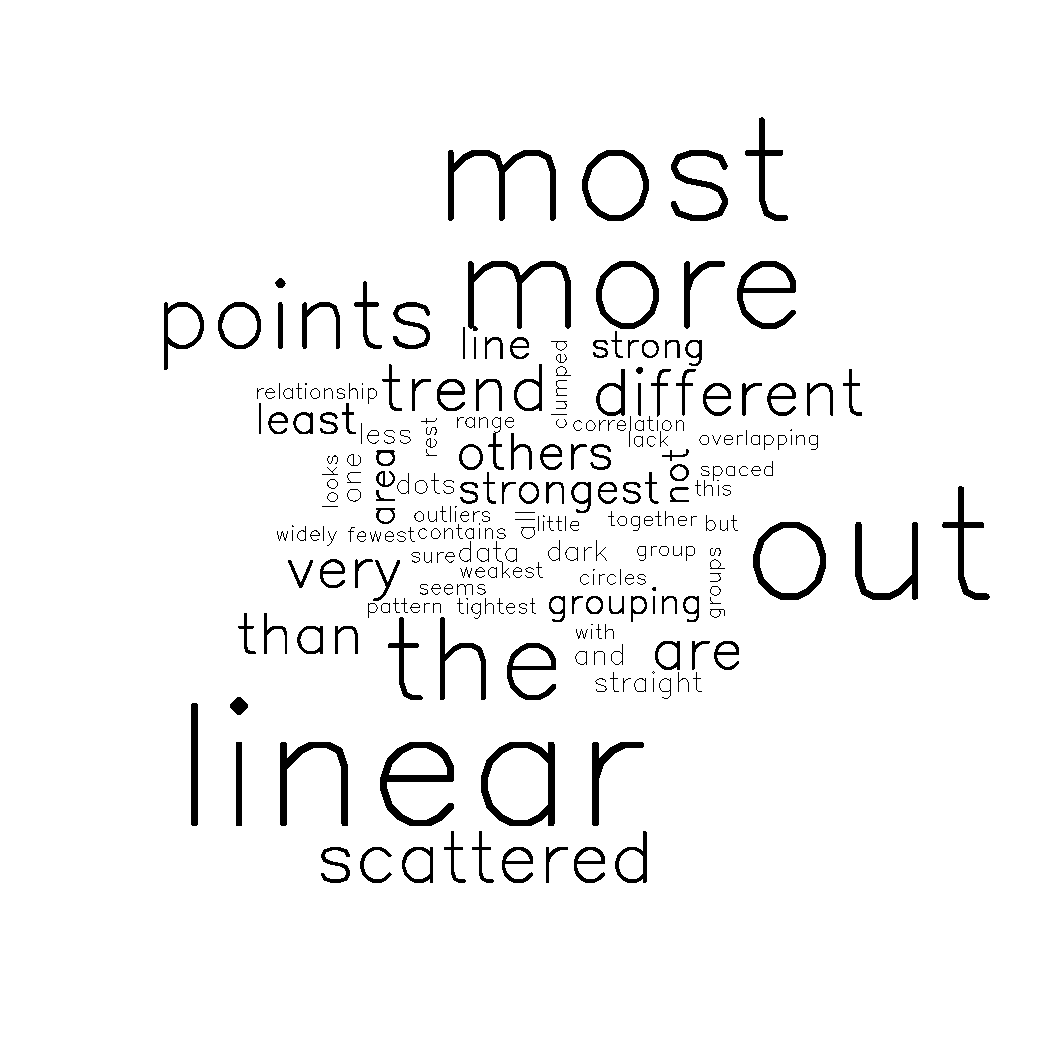
\includegraphics[width=\linewidth]{figure/sentiment-1}
\end{subfigure}
\begin{subfigure}[t]{0.25\linewidth}
  \caption{Plain, cluster target}\vspace{-0.15in}
  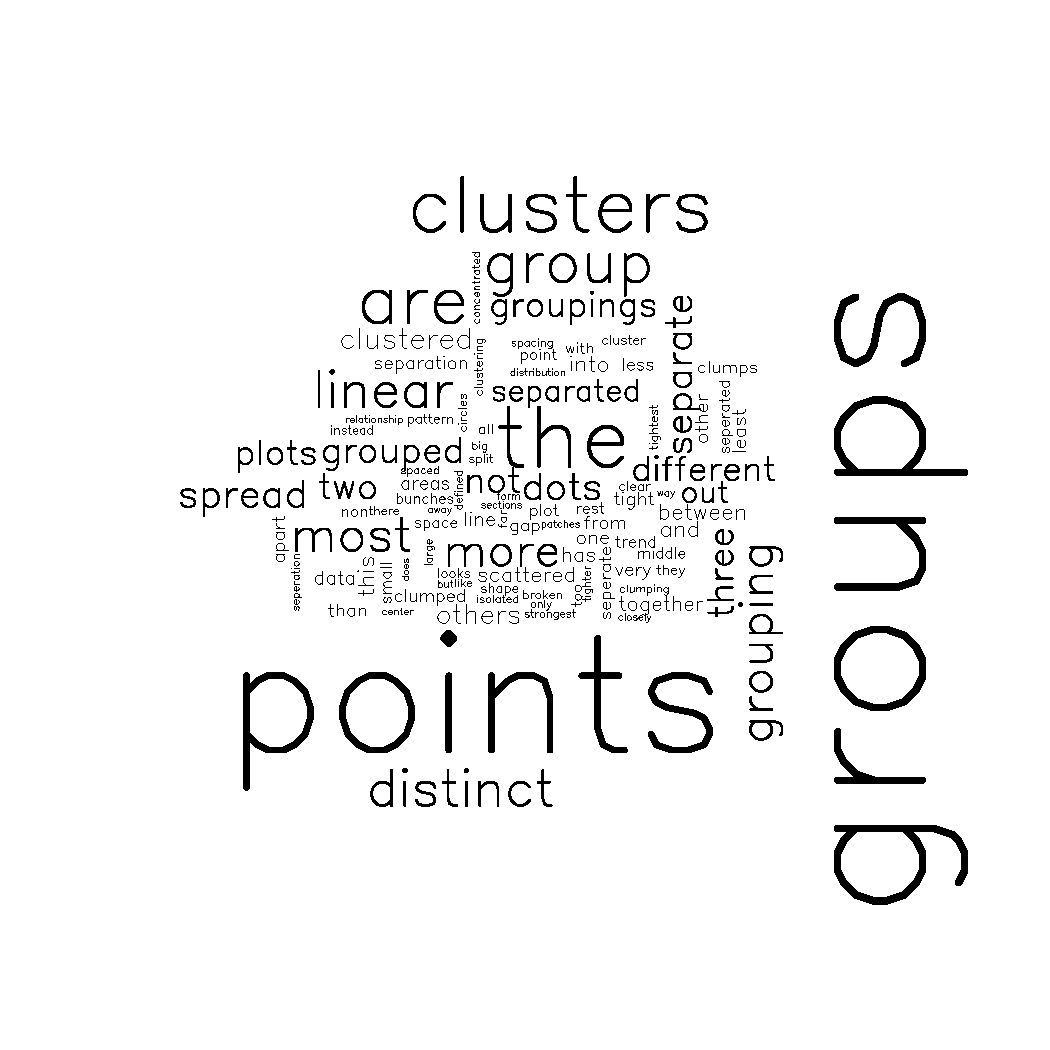
\includegraphics[width=\linewidth]{figure/sentiment-2}
\end{subfigure}
\begin{subfigure}[t]{0.25\linewidth}
  \caption{Plain, trend target}\vspace{-0.15in}
  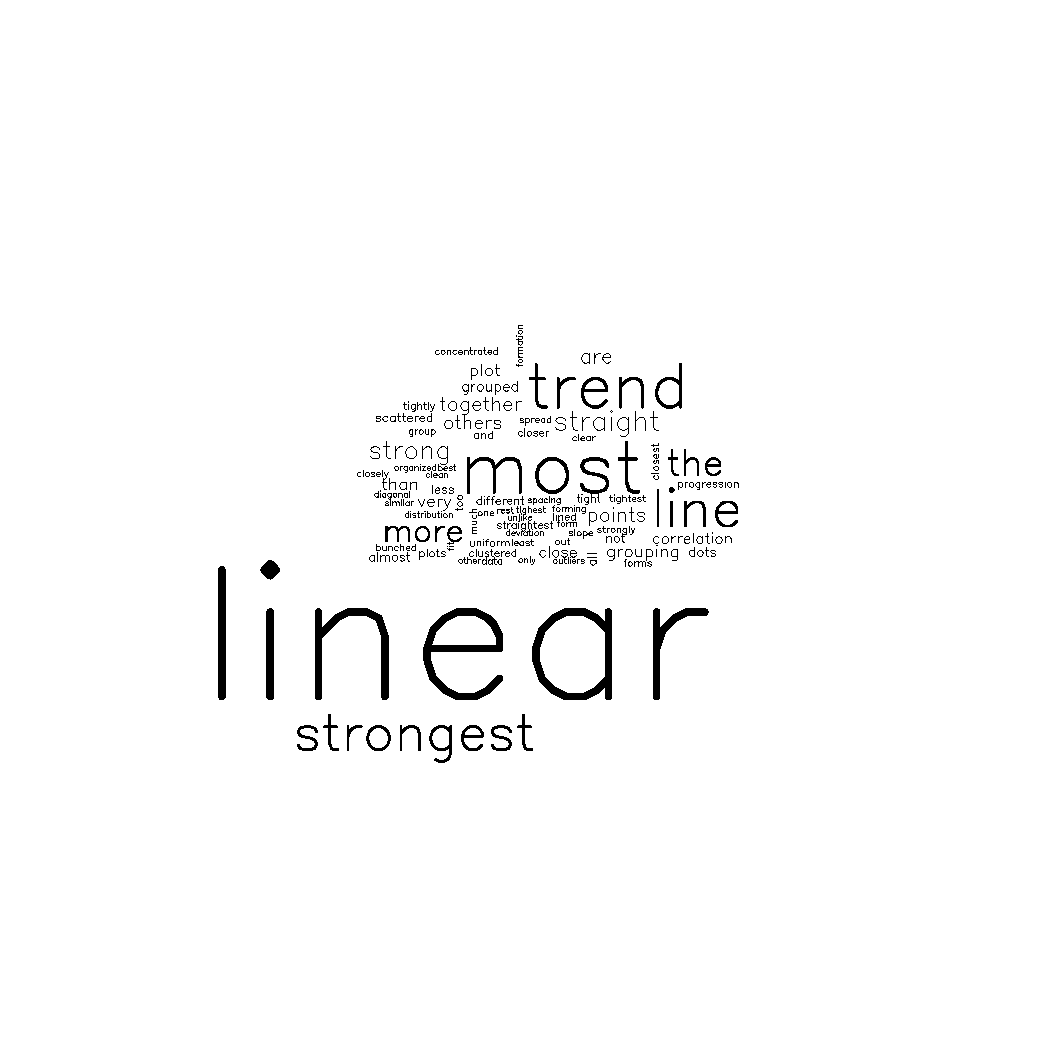
\includegraphics[width=\linewidth]{figure/sentiment-3}
\end{subfigure}

\begin{subfigure}[t]{0.25\linewidth}
  \caption{Trend, neither target}\vspace{-0.2in}
  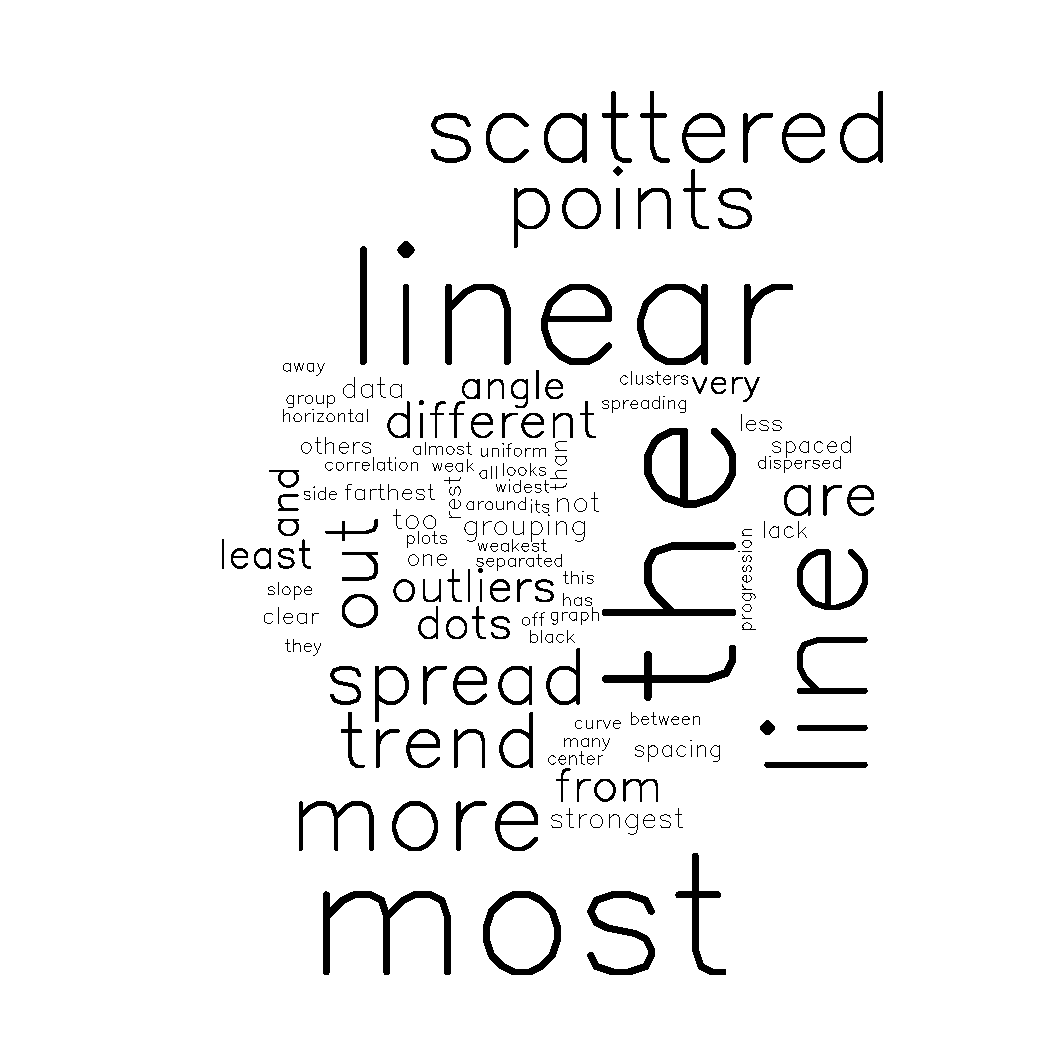
\includegraphics[width=\linewidth]{figure/sentiment-4}
\end{subfigure}
\begin{subfigure}[t]{0.25\linewidth}
  \caption{Trend, cluster target}\vspace{-0.2in}
  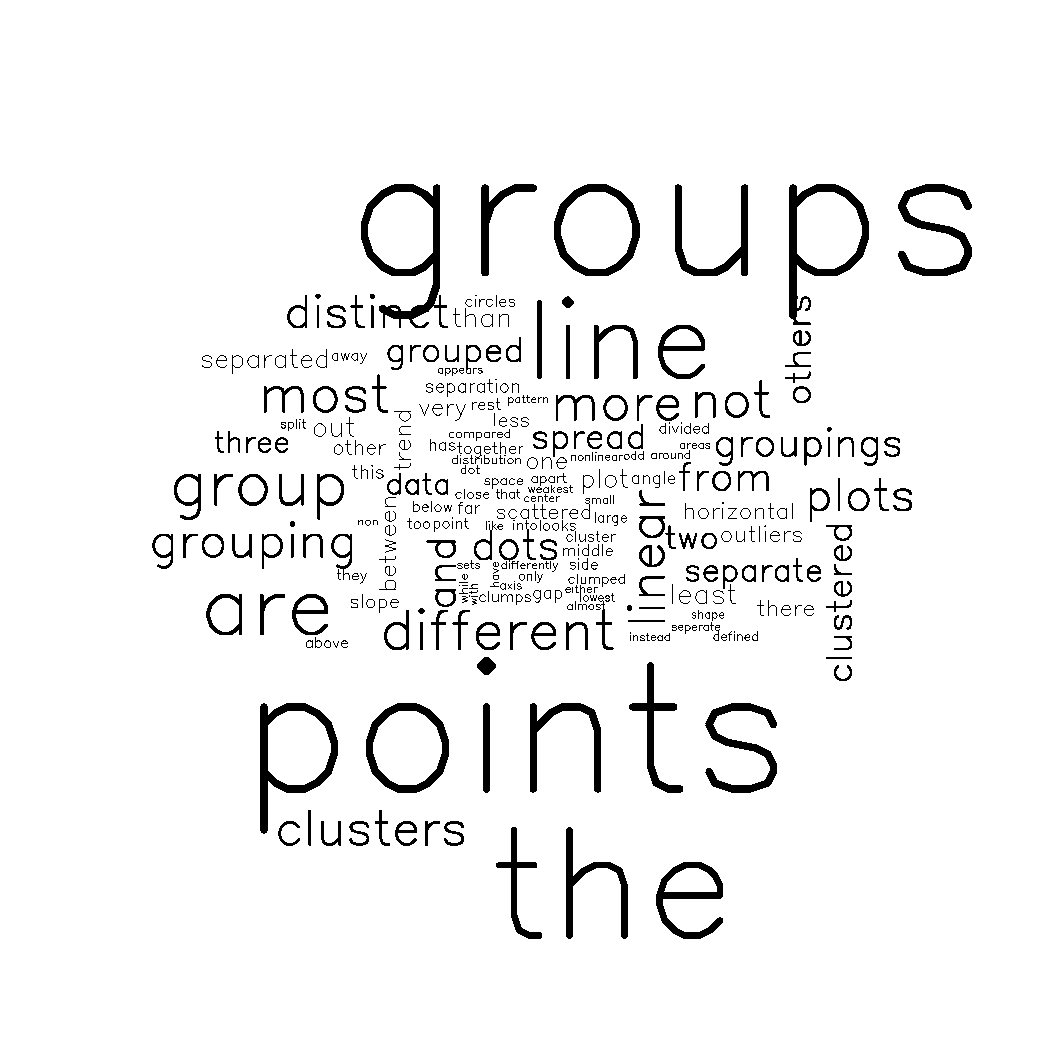
\includegraphics[width=\linewidth]{figure/sentiment-5}
\end{subfigure}
\begin{subfigure}[t]{0.25\linewidth}
  \caption{Trend, trend target}\vspace{-0.2in}
  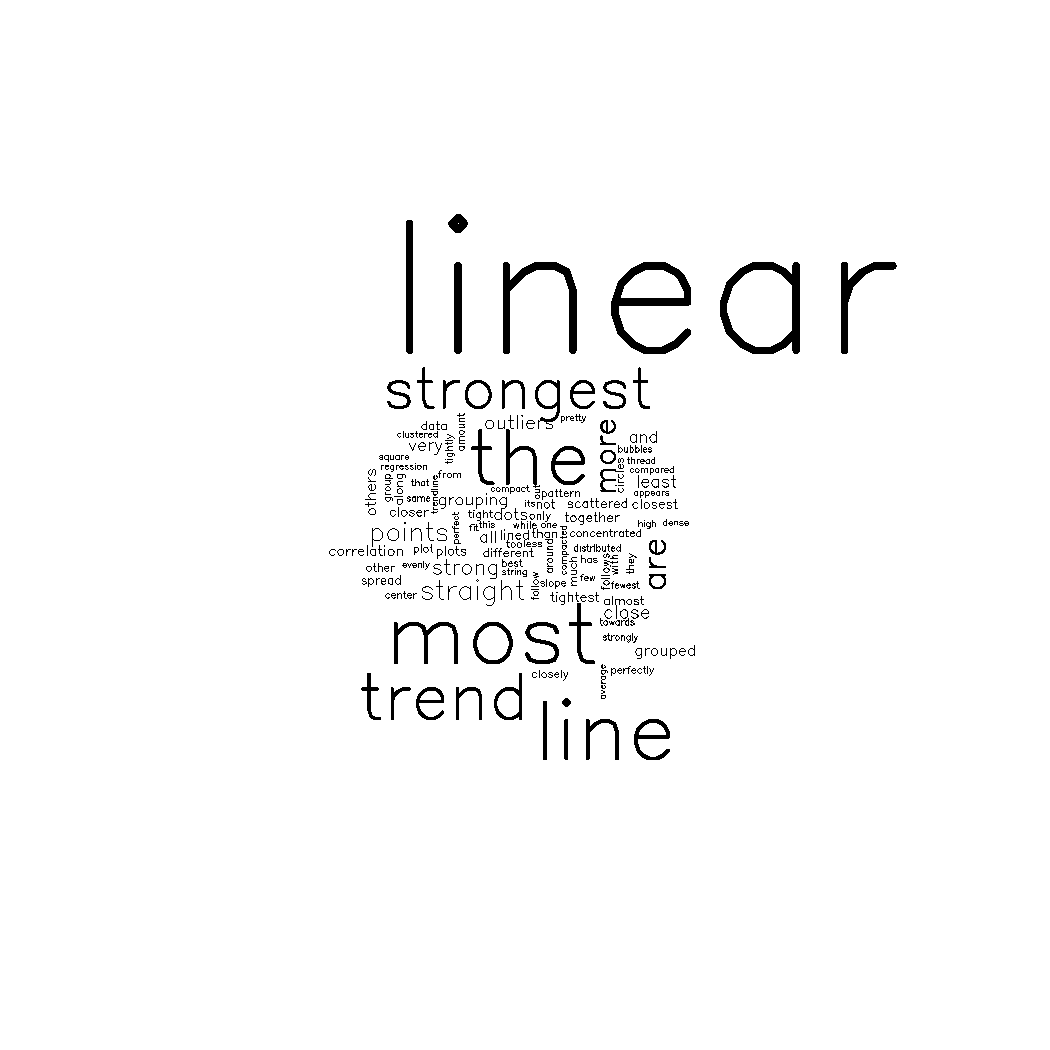
\includegraphics[width=\linewidth]{figure/sentiment-6}
\end{subfigure}

\begin{subfigure}[t]{0.25\linewidth}
  \caption{Color, neither target}\vspace{-0.2in}
  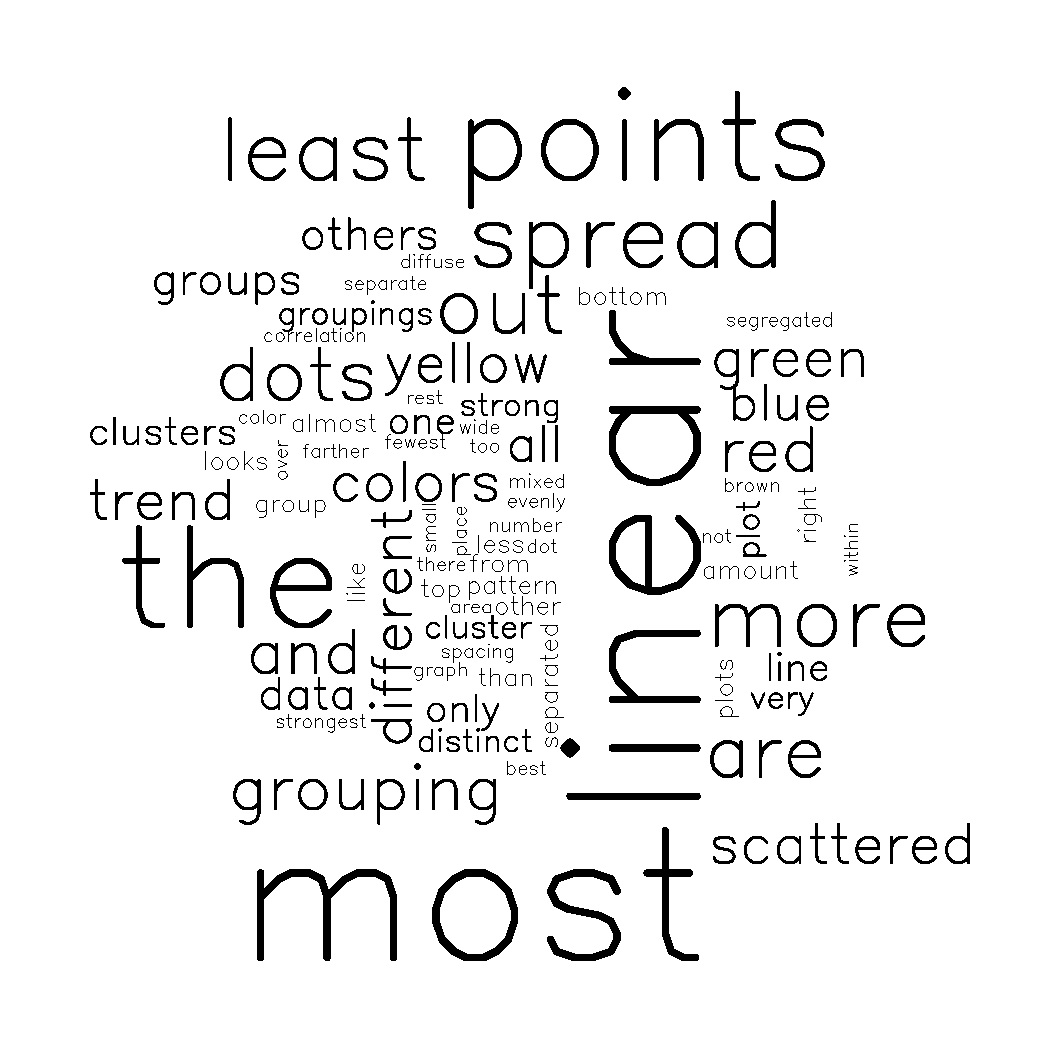
\includegraphics[width=\linewidth]{figure/sentiment-7}
\end{subfigure}
\begin{subfigure}[t]{0.25\linewidth}
  \caption{Color, cluster target}\vspace{-0.2in}
  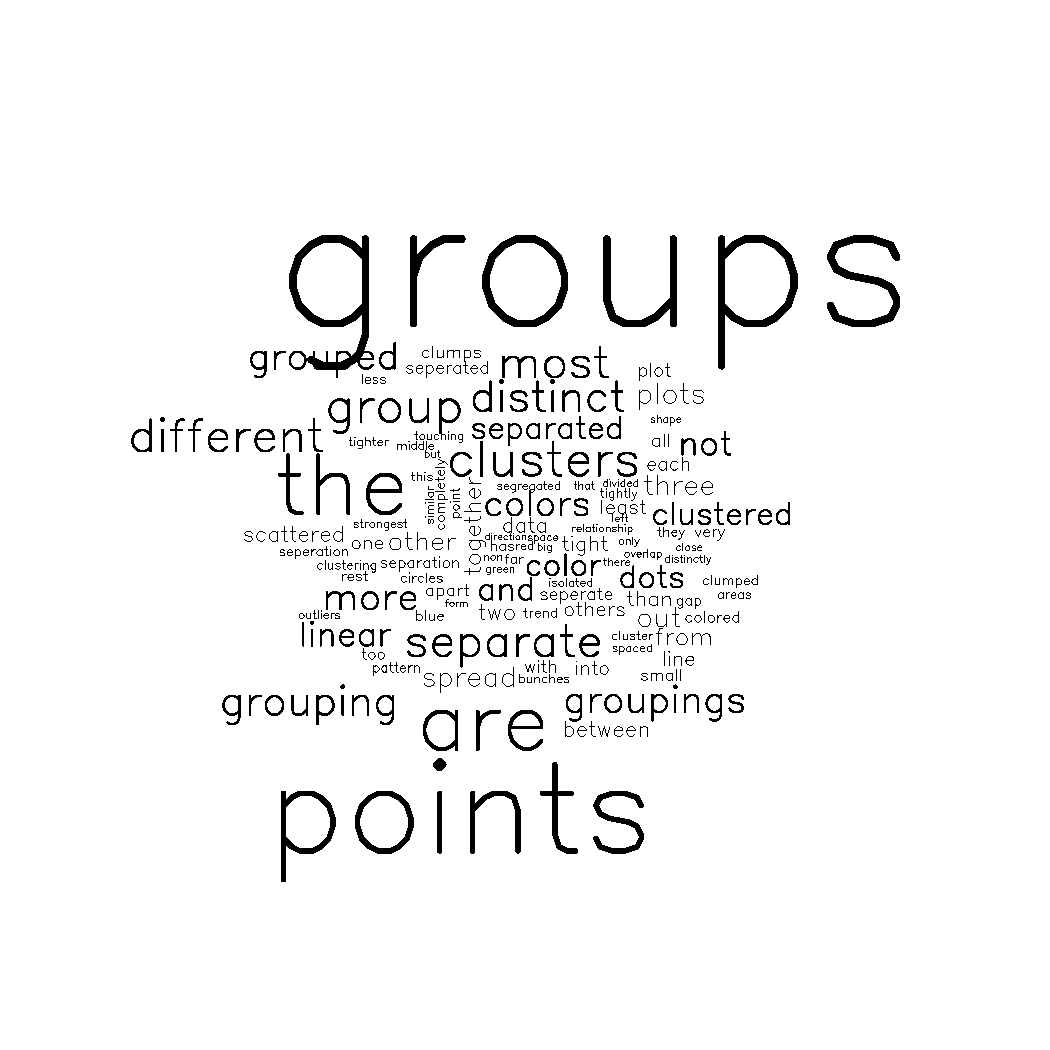
\includegraphics[width=\linewidth]{figure/sentiment-8}
\end{subfigure}
\begin{subfigure}[t]{0.25\linewidth}
  \caption{Color, trend target}\vspace{-0.2in}
  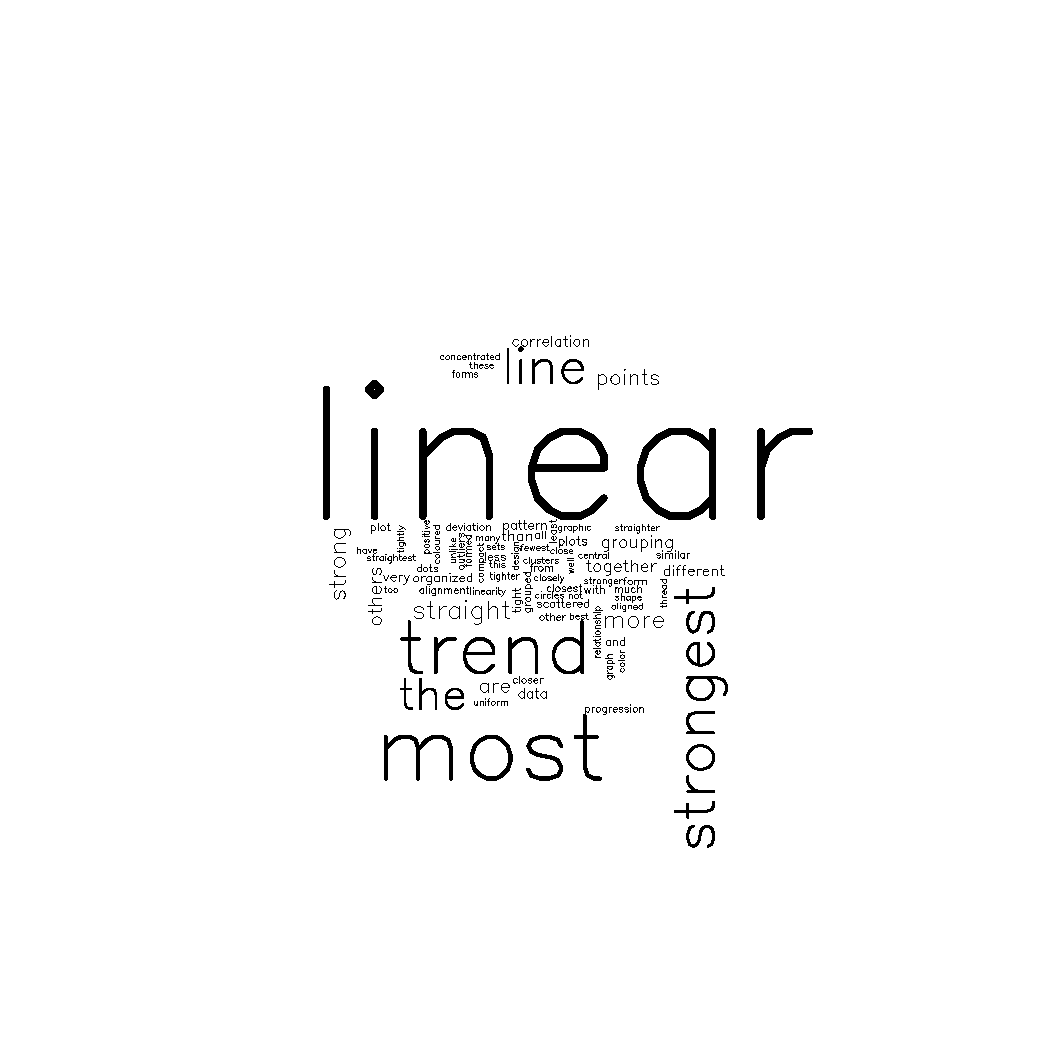
\includegraphics[width=\linewidth]{figure/sentiment-9}
\end{subfigure}

\begin{subfigure}[t]{0.25\linewidth}
  \caption{Color + Ellipse, neither target}\vspace{-0.2in}
  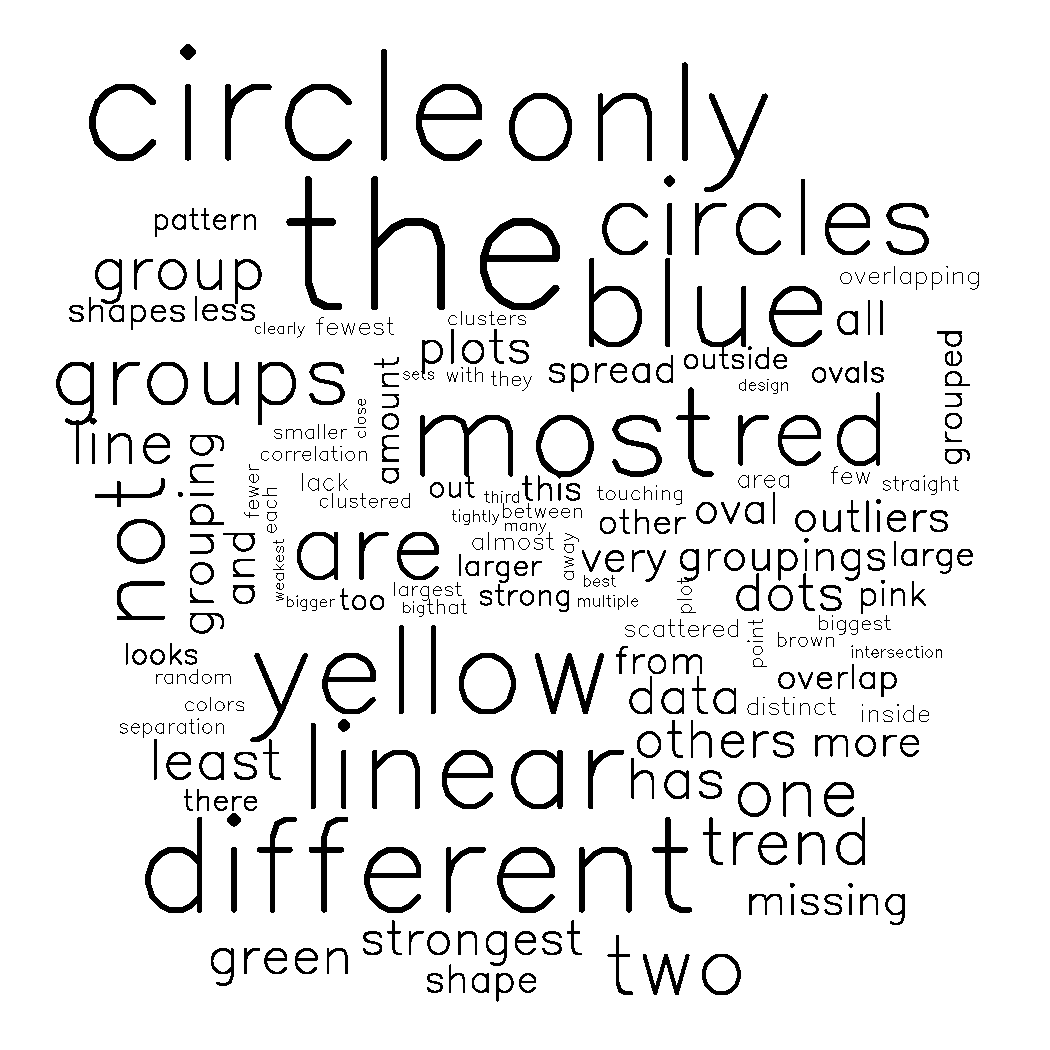
\includegraphics[width=\linewidth]{figure/sentiment-10}
\end{subfigure}
\begin{subfigure}[t]{0.25\linewidth}
  \caption{Color + Ellipse, cluster target}\vspace{-0.2in}
  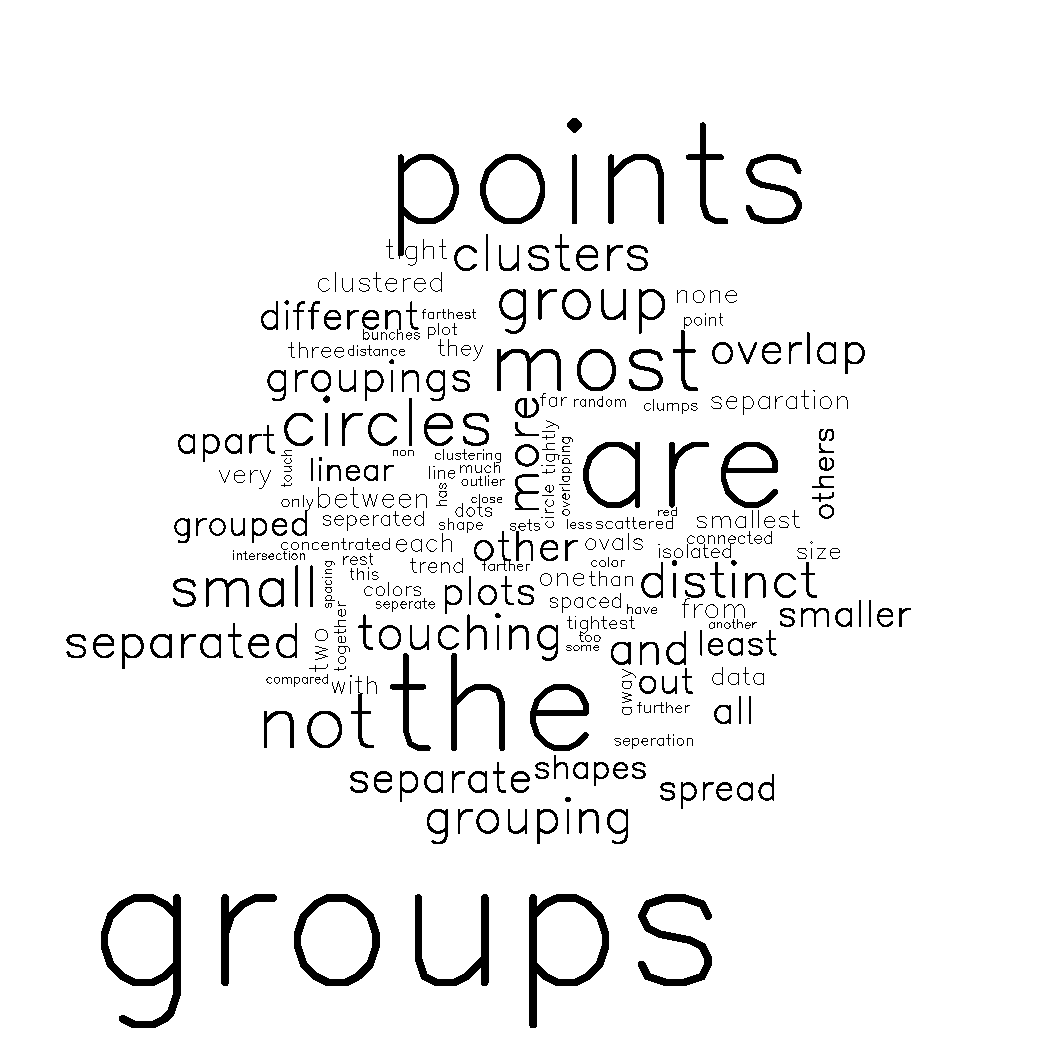
\includegraphics[width=\linewidth]{figure/sentiment-11}
\end{subfigure}
\begin{subfigure}[t]{0.25\linewidth}
  \caption{Color + Ellipse, trend target}\vspace{-0.2in}
  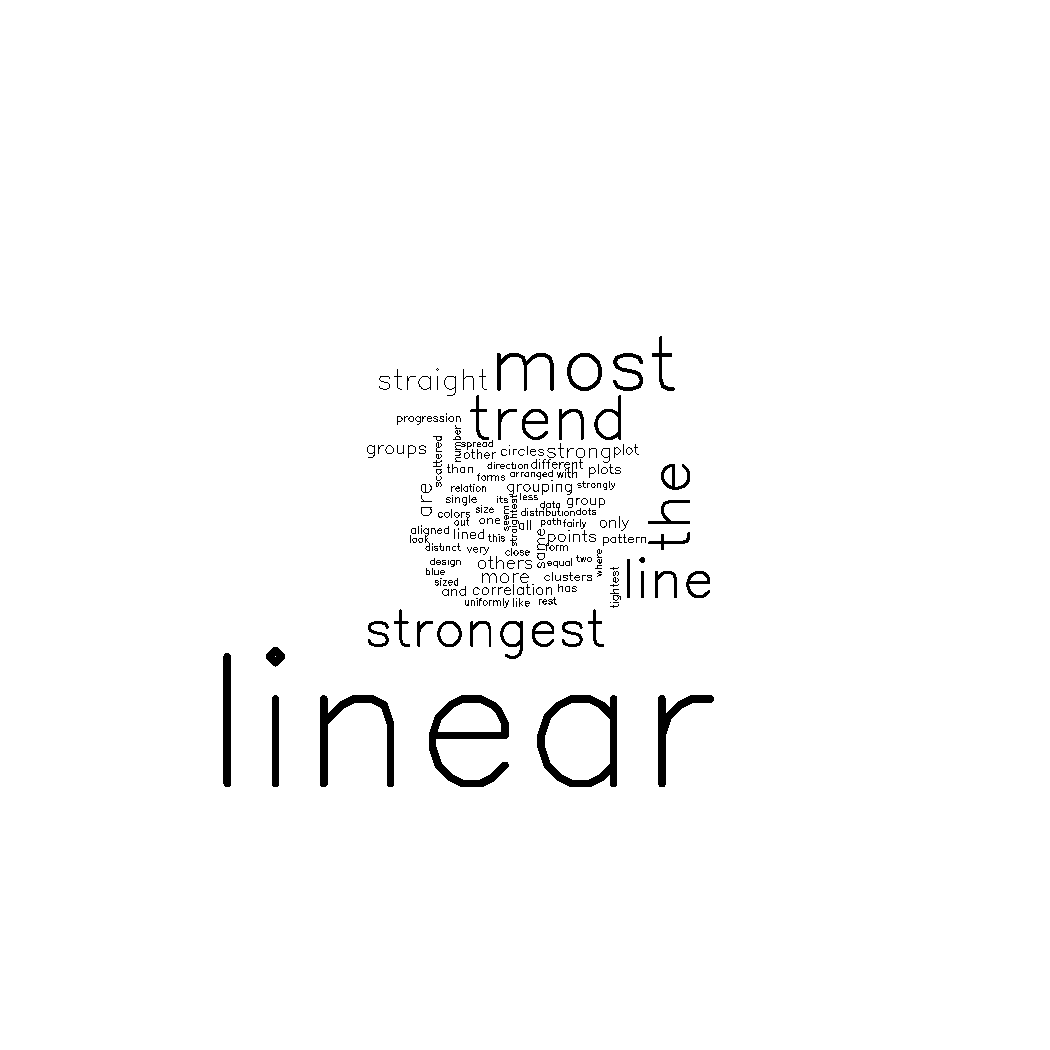
\includegraphics[width=\linewidth]{figure/sentiment-12}
\end{subfigure}
\caption[Wordclouds of participant responses for selected plot types]{\label{fig:wordles}Wordclouds of participants' reasoning by outcome for a selected number of plot types. Mostly, the reasoning and the choice of the target are highly associated. For the Color + Ellipse plot, participants were distracted from either target by an imbalance in the cluster/color distribution, as can be seen from the reasoning in the bottom left wordcloud.}
\end{figure}
\afterpage{\clearpage}
For a more quantitative analysis, responses were categorized based on keywords such as ``line(ar)'', ``correlation'', ``group'', ``cluster'', ``clump'', as well as the presence of negation words (non, not, less, etc.). In addition to linear, nonlinear, and group sentiment, many responses focused on the presence of outliers or the amount of variability present in the chosen plot. 
\begin{figure}[ht]\centering
\begin{knitrout}
\definecolor{shadecolor}{rgb}{0.969, 0.969, 0.969}\color{fgcolor}

{\centering \includegraphics[width=.8\linewidth]{figure/lexical-analysis-1} 

}



\end{knitrout}
\caption[Lexical analysis of participant reasoning]{Lexical analysis of participants' justification of plot selection. Group sentiment in the reasoning is highly associated with selection of the cluster target plot; linear sentiment is highly associated with selection of the trend target plot.}\label{fig:lexicalanalysis}
\end{figure}

\afterpage{\clearpage}
The results of this analysis, shown in Figure~\ref{fig:lexicalanalysis} and supported by Figure~\ref{fig:wordles}, indicate that for the most part participants were making decisions based on the criteria we manipulated; rather than alternate visual cues such as group size. In future studies, however, group size should be more tightly controlled to reduce the presence of distractor aesthetics in null plots. 


\section{Discussion and Conclusions}\label{sec:Conclusion}

Taken together, the results presented suggest that plot aesthetics influence the perception of the dominant effect in the displayed data. This effect is not simply additive (otherwise, the two conflicting aesthetic conditions would result in similarly neutral effects); rather, the effect is consistent with layering of gestalt perceptual heuristics. Plot layers which add additional heuristics show larger effects than plot layers which duplicate heuristics which are already in play. For example, adding ellipses to a plot which has color aesthetics increases group recognition by recruiting the common region heuristic in addition to the point similarity heuristic recruited by color; adding shape to a plot which has color aesthetics may increases group recognition slightly, but does not add additional gestalt heuristics (though point similarity is emphasized through two different mechanisms). 

In order to explicitly rank aesthetics given this nonadditive mechanism, it would be necessary to test ellipse and error band aesthetics alone; in this study, we have only examined those aesthetics in combination with color and regression line plot layers, as the bounding aesthetics are seldom seen alone. 

While further studies are necessary to control for the effects of cluster size as well as to explore the gestalt heuristics applicable to other types of plots, these results demonstrate the importance of carefully constructing graphs in order to consistently convey the most important aspects of the displayed data. 


\bibliographystyle{asa}
\bibliography{references}
\newpage
\begin{appendix}
\section{Simulation Studies of Parameter Space}\label{app:parametersimulation}

Using 1000 simulations for each of the 98 combinations of parameters ($K=\{3,5\}$, $\sigma_C=\{.1, .15, .2, .25, .3, .35, .4\}$, $\sigma_T=\{.2, .25, .3, .35, .4, .45, .5\}$), we explored the effect of parameter value on the distribution of summary statistics describing the line strength ($R^2$) and cluster strength for null and target plots. 

Figures \ref{fig:simulationLineIntervals} and \ref{fig:simulationClusterIntervals} show the 25th and 75th percentiles of the distribution of $R^2$ and cluster strength summary statistics for each set of parameter values. These plots guided our evaluation of ``easy", ``medium" and ``hard" parameter values for line and cluster tasks. 

Additionally, we note that there is an interaction between $\sigma_C$ and $\sigma_T$: the distinction between target and null on a fixed setting of clustering becomes increasingly difficult as the standard deviation for the linear trend is increased, and vice versa. There may additionally be a three-way interaction between $\sigma_C, \sigma_T$, and $K$: the size of the blue intervals (bottom figure) changes in size between different levels of $K$, it changes for different levels of $\sigma_C$ and $\sigma_T$. These interactions suggest that in order to examine differences in aesthetics, we must block by parameter settings (this can be accomplished through blocking by dataset). Each dataset is non-deterministic, because we have a random process generating from different parameter settings, not a deterministic run setting as in an engineering setting. It is thus important to use replicates of each parameter setting to ensure that we can separate data-level effects from parameter-level effects. 



\begin{figure}[ht]\centering
\includegraphics[width=.8\linewidth]{figure/simulationparameters-1}
\caption{Simulated interquartile range of $R^2$ values for target and null data distributions. \label{fig:simulationLineIntervals}}
\end{figure}

\begin{figure}[ht]\centering
\includegraphics[width=.8\linewidth]{figure/simulationparameters-2}
\caption{Simulated interquartile range of cluster cohesion statistic values for target and null data distributions. \label{fig:simulationClusterIntervals}}
\end{figure}

Additionally, after the experiment was complete, we examined the distribution of group size (as measured by gini impurity) to establish whether there were any systematic differences in group size inequality between data generated from $M_0$ (null data) and data generated from $M_C$ (cluster data). Figure~\ref{fig:simulationGiniIntervals} demonstrates that the cluster plots have significantly lower group size differences than null plots at all parameter combinations. It is therefore possible that some participants will identify extraordinarily unequal group sizes present in null plots as significantly different from the other lineup plots, ignoring any cluster signal. Future studies should more tightly control group size in order to reduce this effect. 

\begin{figure}[ht]\centering
\includegraphics[width=.8\linewidth]{figure/simulationparameters-3}
\caption{Simulated interquartile range of group size inequality statistic values for cluster and null data distributions. \label{fig:simulationGiniIntervals}}
\end{figure}

\section{Model Results}
\subsection{Trend Model Results}\label{app:trendmodel}
\input{figure/linear-fixef-table}
\subsection{Cluster Model Results}\label{app:clustermodel}
\input{figure/group-fixef-table}


\subsection{Is difficulty of Lineups matching with parameter settings? *** out? appendix? ***}

\newdo{We should look at the percentages and match them with the actual numeric values of the indices in the data.}

\newdo{Figure~\ref{cluster-trend} shows the percentages of correct data identification in plain plots facetted by trend/cluster parameter. For $K=5$ the identification is negatively impacted by a higher variability, as it should be. 
What we still need to include is the actual cluster/trend index for each of the data sets, and compare that to the percentages. (This is done in ParameterAnalysis.R and should be copied in here.) 
All of the (plain plottype) lineups are hugely significant (less than 1 in 10,000 events), i.e.\ participants reliably identify at least one of the targets as different from the other panels. We can therefore go directly into the conditional analysis of section \ref{sec:faceoff}.
}



\begin{figure}
\centering
\begin{knitrout}
\definecolor{shadecolor}{rgb}{0.969, 0.969, 0.969}\color{fgcolor}

{\centering \includegraphics[width=0.5\textwidth]{figure/unnamed-chunk-1-1} 

}



\end{knitrout}
\caption{\label{cluster-trend} Overall, the percentages of correct data identifications match variability (i.e.\ they decrease as variability increases - the above plot shows results from plain plots only). }
\end{figure}

\begin{figure}
\centering
\begin{knitrout}
\definecolor{shadecolor}{rgb}{0.969, 0.969, 0.969}\color{fgcolor}

{\centering \includegraphics[width=0.5\textwidth]{figure/unnamed-chunk-2-1} 

}




{\centering \includegraphics[width=0.5\textwidth]{figure/unnamed-chunk-2-2} 

}



\end{knitrout}
\caption{\label{clusters.and.trends} For future reference - as the difference between the signals increases, the chance that an observer picks the corresponding target increases.}
\end{figure}






\subsection{Single Target Plot Models *** out ***}

We  model the probability of selecting the target plot using a logistic regression with plot type as a fixed effect, and random effects for dataset (which encompasses parameter effects) and participant (accounting for variation in individual skill level). 

For plot type $i$, displaying dataset $j=1, ..., 54$ and participant $k=1, ..., P$, we model

\begin{align}
\text{logit }P(\text{success}) & =  \textbf{X}\beta + \textbf{J}\gamma + \textbf{K}\eta + \epsilon, \label{eqn:linearModel}\\
\text{where } \beta_i & \hphantom{\sim} \text{describe the effect of specific plot aesthetics}\nonumber\\
\hphantom{where } \gamma_j & \overset{iid}{\sim} N\left(0, \sigma^2_{\text{data}}\right)\text{, the random effect for dataset specific characteristics}\nonumber\\
\hphantom{where } \eta_k & \overset{iid}{\sim} N\left(0, \sigma^2_{\text{participant}}\right)\text{, the random effect for participant characteristics}\nonumber\\
\text{and } \epsilon_{ijk} & \overset{iid}{\sim}  N\left(0, \sigma^2_e\right)\text{, the error associated with a single trial evaluation} \nonumber
\end{align}

We note that any variance due to parameters $K$, $\sigma_T$, and $\sigma_C$ is contained within $\sigma^2_{\text{data}}$ and can be examined using a subsequent model. 

\subsubsection{Linear Target Model}



We define success as ``the participant correctly identified the trend target plot generated by $M_T$" and use this as dependent variable in model equation (\ref{eqn:linearModel}).  Figure~\ref{fig:linear.fixef} shows the fixed effects of the resulting model fit. Color, Shape, and Ellipse aesthetics (and combinations thereof) decrease participant recognition of the trend target plot, while the Trend + Error combination increases participant recognition of the trend target plot.

These results are consistent with our hypothesis that aesthetics which emphasize the gestalt similarity heuristic decrease recognition of the trend target plot. The aesthetic combinations of color + shape + ellipse and color + ellipse, which recruit gestalt heuristics for similarity and common region, strongly reduce the probability of detecting the trend target plot. Aesthetic combinations which only activate the gestalt similarity heuristic, such as color, shape, and color+shape, have somewhat less of an effect. As would be predicted by previous studies, such as \citet{lewandowsky1989discriminating}, color (or color + shape) more strongly detracts from trend target recognition than shape alone. 

The trend line aesthetic does not significantly increase trend target plot recognition, either alone or in the conflict condition color + trend. This may be because the gestalt heuristic recruited in this case is good continuation (``two elements which blend together smoothly likely belong to one unit"), the same heuristic recruited by the points alone. Thus, the trend line may provide only slight additional visual emphasis from the gestalt perspective.


\begin{figure}[htbp]\centering
\begin{knitrout}
\definecolor{shadecolor}{rgb}{0.969, 0.969, 0.969}\color{fgcolor}

{\centering \includegraphics[width=.75\linewidth]{figure/line-fixef-1} 

}



\end{knitrout}
\caption{Odds of detecting the linear target plot for each aesthetic. Only the combination of Trend + Error significantly increases the odds of linear target plot detection relative to the control plot (plain scatterplot). \label{fig:linear.fixef}}
\end{figure}
\afterpage{\clearpage}

\newdo{at the moment I can not imagine an error band that would involve connectedness. I don't think you ever mentioned connectedness in the talks ... could we leave this out to clean the argument up?}
Once error bands are added to the plot, the continuity and common region heuristics may be applied. The results are consistent with this idea: only the dual continuity emphasis of trend + error bands (along with the common region emphasis) significantly increases the probability that participants will identify the target plot generated under $M_T$. 


\subsubsection{Cluster Target Selection *** keep some of the cognitive discussion ***}\label{sec:groupModel}


We now examine the probability of selecting the cluster target plot as a function of plot type, with random effects for dataset (which encompasses parameter effects) and participant (accounting for variation in individual skill level). The model fit here is the same as that shown in equation \eqref{eqn:linearModel}, except that the dependent variable in this model is defined as the successful identification of the cluster target plot. 

\begin{figure}[ht]\centering
\begin{knitrout}
\definecolor{shadecolor}{rgb}{0.969, 0.969, 0.969}\color{fgcolor}

{\centering \includegraphics[width=.75\linewidth]{figure/group-fixef-1} 

}



\end{knitrout}
\caption{Odds of detecting the cluster target plot for each aesthetic, relative to a plain scatterplot. The presence of error lines or bounding ellipses significantly decreases the probability of correct target detection, and no aesthetic successfully increases the probability of correct target detection. This may be due to differences in cluster size for null plots, with data generated under $M_0$ compared with the group target plot displaying data generated under $M_C$. \label{fig:group.fixef}}
\end{figure}


Figure~\ref{fig:group.fixef} contains odds and 95\% Wald intervals of the estimated fixed effects obtained by fitting equation \ref{eqn:linearModel} to a binary indicator of successful cluster target identification. 
According to the model results, no plot aesthetics significantly increase the odds of selecting the group target plot compared to the plain design; however, several aesthetic combinations decrease the odds. Consistent with our hypothesis,  Color + Ellipse + Trend + Error and Trend + Error plot aesthetic combinations significantly decrease the detection of the group target plot. 

However, the implication that Color + Ellipse and Color + Shape + Ellipse also decrease group target detection is not consistent with our hypotheses. Examination of participants' reasons for selecting specific target plots provides at least some explanation; participants cited reasons such as 
``There is no circle highlighting the yellow symbols in this plot" %line 13515 
and 
``Lack of a circle around the red symbols".  %line 13516

This suggests that our cluster allocation for null target plots may have produced unintentional results; rather than providing unambiguous gestalt cues which reinforced group separation, our null plots provided mixed cues which varied the number of points in a cluster and the presence of the additional similarity cue. 
Numerically, these null data sets had uneven cluster allocation; bounding ellipse estimation failed for groups with fewer than three points and in these cases, ellipses were not drawn. 
Visually, the conspicuous absence of an ellipse will lead participants to select null plots with that feature (see section~\ref{sec:sentiment} for a more detailed look at participants' responses).
In particular, counting is pre-attentive, and the number of ellipses in each plot is within some estimates of the `subitizing' range of counting, which can be counted without spatial attention \citep{trick1994small}. Thus, the number of ellipses present dominates other features which are important for gestalt grouping heuristics. 

% \newdo{Counting and estimation is one of the pre-attentive tasks (besides target detection, boundary detection, and region tracking) that studies have identified, for an overview see \url{http://www.csc.ncsu.edu/faculty/healey/download/tvcg.11.pdf} (Healey's TVCG paper corresponding to his website on the overview of pre-attentiveness). }

This effect actually provides some additional information as to the hierarchy of gestalt features: for plots displaying the same data (including at least one plot with cluster size of fewer than three points), participants were more likely to identify the cluster target plot under the Color and Shape aesthetics than under Color + Ellipse or Color + Shape + Ellipse conditions. 
The presence of the ellipse (and the gestalt common region heuristic) dominated the effect of point similarity (albeit not in the way the authors originally intended). 
In future experiments, it will be advantageous to control the variability in cluster size in order to remove the conflicting visual influence of gestalt common region heuristics with the greater similarity and proximity present in the target plot. 

\subsection{Response Time *** out ***}
As data collection was conducted entirely online, we cannot measure responses in the millisecond range characteristic of many psychometric studies, however, the data server does record the time between initial lineup presentation (trial start) and answer submission (trial end). 
Examining differences in average response times across trials provides us with an additional measure of trial difficulty or perceptual complexity. 
We can also explore whether participants spent more time on certain types of plots and how additional time is realted to accurate target identification. 

\begin{figure}[ht]\centering
\begin{knitrout}
\definecolor{shadecolor}{rgb}{0.969, 0.969, 0.969}\color{fgcolor}

{\centering \includegraphics[width=\linewidth]{figure/timemodel-plottype-1} 

}



\end{knitrout}
\caption{\label{fig:timemodel-aes} Results of a model describing log evaluation time by evaluation outcome and plot type. Participants take less time to evaluate plots with a single aesthetic compared with more complicated plots. }
\end{figure}

We model log-transformed reaction time as a function of evaluation outcome (neither target identified, cluster or trend target identified, or both targets identified) and plot type. In order to remove the ``novelty" effect of an unfamiliar task, we also include an indicator variable for the first trial an individual completed \citep{Majumder:2014up}. A random effect for participant and dataset is included to account for the experimental design. Figure~\ref{fig:timemodel-aes} displays the model results for each outcome of the lineup evaluation; simple plots (color, trend, shape) take less time to evaluate (across all conditions) than plots with more than one aesthetic. Additionally, participants who identified the cluster target took less time (in most cases) than participants identifying the trend target.  

\begin{figure}[ht]\centering
\begin{knitrout}
\definecolor{shadecolor}{rgb}{0.969, 0.969, 0.969}\color{fgcolor}\begin{kframe}


{\ttfamily\noindent\bfseries\color{errorcolor}{\#\# Error in `\$<-.data.frame`(`*tmp*`, "{}estimate"{}, value = structure(c(0.577833500194697, : replacement has 69 rows, data has 71}}

{\ttfamily\noindent\bfseries\color{errorcolor}{\#\# Error in `\$<-.data.frame`(`*tmp*`, "{}name"{}, value = c("{}simpleoutcomeneither:trend.diffeasy:cluster.diffeasy:k3"{}, : replacement has 69 rows, data has 71}}

{\ttfamily\noindent\bfseries\color{errorcolor}{\#\# Error in strsplit(coefs\$name, split = "{}:"{}): non-character argument}}

{\ttfamily\noindent\bfseries\color{errorcolor}{\#\# Error in `\$<-.data.frame`(`*tmp*`, "{}outcome"{}, value = c("{}neither"{}, "{}cluster"{}, : replacement has 39 rows, data has 71}}

{\ttfamily\noindent\bfseries\color{errorcolor}{\#\# Error in `\$<-.data.frame`(`*tmp*`, "{}trend.diff"{}, value = c("{}plottypeplain"{}, : replacement has 39 rows, data has 71}}

{\ttfamily\noindent\bfseries\color{errorcolor}{\#\# Error in `\$<-.data.frame`(`*tmp*`, "{}trend.diff"{}, value = structure(integer(0), .Label = c("{}Trend:Easy"{}, : replacement has 0 rows, data has 71}}

{\ttfamily\noindent\bfseries\color{errorcolor}{\#\# Error in `\$<-.data.frame`(`*tmp*`, "{}cluster.diff"{}, value = character(0)): replacement has 0 rows, data has 71}}

{\ttfamily\noindent\bfseries\color{errorcolor}{\#\# Error in `\$<-.data.frame`(`*tmp*`, "{}cluster.diff"{}, value = structure(integer(0), .Label = c("{}Cluster:Easy"{}, : replacement has 0 rows, data has 71}}

{\ttfamily\noindent\bfseries\color{errorcolor}{\#\# Error in `\$<-.data.frame`(`*tmp*`, "{}k"{}, value = character(0)): replacement has 0 rows, data has 71}}

{\ttfamily\noindent\bfseries\color{errorcolor}{\#\# Error in `\$<-.data.frame`(`*tmp*`, "{}simple"{}, value = integer(0)): replacement has 0 rows, data has 71}}

{\ttfamily\noindent\bfseries\color{errorcolor}{\#\# Error in `\$<-.data.frame`(`*tmp*`, "{}simple"{}, value = structure(integer(0), .Label = character(0), class = "{}factor"{})): replacement has 0 rows, data has 71}}

{\ttfamily\noindent\bfseries\color{errorcolor}{\#\# Error in levels(coefs\$simple) <- c("{}Neither"{}, "{}Cluster, Trend"{}, "{}Both"{}): attempt to set an attribute on NULL}}

{\ttfamily\noindent\bfseries\color{errorcolor}{\#\# Error in `\$<-.data.frame`(`*tmp*`, "{}outcome"{}, value = structure(integer(0), .Label = c("{}Neither Identified"{}, : replacement has 0 rows, data has 71}}

{\ttfamily\noindent\bfseries\color{errorcolor}{\#\# Error in `\$<-.data.frame`(`*tmp*`, "{}pos"{}, value = numeric(0)): replacement has 0 rows, data has 71}}

{\ttfamily\noindent\bfseries\color{errorcolor}{\#\# Error in eval(expr, envir, enclos): object 'outcome' not found}}\end{kframe}
\end{knitrout}
\caption{\label{fig:timemodel-pars} Results of a model describing log evaluation time by evaluation outcome, plot type, data-generation parameters, and participant experience. }
\end{figure}
\input{figure/timemodel-pars-fixef-table}

In a second model, we fit log response time as a function of the plot type, first trial, and the interaction between the outcome and data-generation parameters $\sigma_C$, $\sigma_T$, and $K$. In order to model the task as designed, we have coded $\sigma_C$ and $\sigma_T$ according to difficulty level - easy, medium, and hard, rather than modeling the numerical parameters themselves; this allows us to describe the psychological task rather than the numerical task (and also simplifies the model slightly). Figure~\ref{fig:timemodel-pars} shows the estimated difference in time as a function of difficulty level and trial outcome, and table \ref{tab:timemodel-pars} shows the additional fitted effects and 95\% intervals which are not shown graphically. 
The time to evaluate each plot increases slightly with trend difficulty and cluster difficulty (across trials), conditional on outcome, but the "medium" difficulty trials seem to be somewhat discordant in many cases; in some cases, time to evaluate increases and in others, it decreases. This may be due to a conflict between the trend and cluster target plots: when there is no clear signal numerically, evaluation time increases while participants waver between potential targets. 

\subsection{Participant Confidence *** out ***}
In addition to participant identification of target plots, we also asked participants to rate their confidence in their answer. 
Figure~\ref{fig:conflevel} shows aggregate participant confidence rating as a function of trial outcome. 
Participants who did not identify either target plot were less likely to be ``extremely confident'' in their answer, while participants who identified either the trend or the cluster target correctly were highly confident that their answer was correct. 
Overall, though, participants seem to have some degree of confidence in their answer, regardless of whether the answer was correct.

\begin{knitrout}
\definecolor{shadecolor}{rgb}{0.969, 0.969, 0.969}\color{fgcolor}\begin{figure}

{\centering \includegraphics[width=.5\linewidth]{figure/participant-confidence-1} 

}

\caption{Participant confidence levels compared with trial results. \label{fig:conflevel}}\label{fig:participant-confidence}
\end{figure}


\end{knitrout}

\section{Simulation based inference in a two-target lineup scenario}\label{sec:simulation}

Assume that there are two targets embedded in a lineup of overall size $m$, where $m$ in our experiment is taken to be $m=20$. Let $A$ be the event that one of these targets is chosen.
Under the null hypothesis that both targets are consistent with being created based on data from the null model, we can assume that under the null hypothesis the expected value of the probability that an observer picks one of these plots from the lineup is $2/m = E[ P(A \mid H_o) ]$.
For the distribution of $A \mid H_o$ we employ a simulation-based strategy:
Under the null hypothesis, we can assume, that the $p$-value corresponding to a hypothesis test `the presented data is consistent with the null model' has a standard uniform distribution, i.e. $p_i \sim U[0,1]$ i.i.d.~for all $1 \le i \le m$. We assume that the choice observers make can be modeled using a multinomial distribution, where the probability $\pi_i$ to pick panel $i$ is inversely linear to $p_i$, with $\sum_{i=1}^m \pi_i = 1$.
 
W.l.o.g.~we can assume that the two target plots are in positions 1 and 2. 
Given that a lineup was evaluated by $K$ individuals, the simulation process for $P(A|H_o$ is then as follows:
%
\begin{enumerate}
\item Pick two values $p_i \sim U[0,1], i=1, 2$.
\item Repeat $b_1$ times:
\begin{enumerate}
    \item Pick $m-2$ values $p_i \sim U[0,1], i=3, ..., m$.
    \item Pick $K$ values from a Multinomial distribution with $\pi = \frac{1-p}{|| 1- p||}$, i.e. $x_j \sim M_\pi, i=1, ..., K$
    \item Return the number of times that $x_j$ is 1 or 2. 
\end{enumerate} 
\end{enumerate}
Repeat the above process $b_2$ times, and average results for a distribution of $A \mid H_o$. 
The choice of $b_1$ and $b_2$ decides on the number of decimal places to which the estimated distribution can be used reliably. 

\begin{figure}

\begin{knitrout}
\definecolor{shadecolor}{rgb}{0.969, 0.969, 0.969}\color{fgcolor}

{\centering \includegraphics[width=0.7\linewidth]{figure/twotarget-1} 

}



\end{knitrout}
\caption{\label{fig:simulation} Ten simulations of size $b_2 = 1,000$ and $b_1 = 100$ for lineups of size $m=20$ assuming $K=10$ evaluations. The averages of the ten simulation runs are shown as lines. The crosses are probabilities from  Binomial $B_{2/20, 10}$.}
\end{figure}
\end{appendix}
\end{document}
